% !TeX program = xelatex
% (C) Hans Wan, Windy Deng
% Licensed under CC BY-NC-SA 4.0 International license.
% This is the LaTeX source code of Your Missing Semester of Using Computer (PDF Version).

\documentclass[a4paper]{book}
\usepackage{missing}

\date{\today}

\begin{document}

\pagenumbering{Alph}
\maketitle

\frontmatter
\pdfbookmark{内封}{innertitle}
\thispagestyle{empty}
\begin{center}
  \vspace*{2.5cm}
  \fontsize{42pt}{54pt}\selectfont{}\textsf{你缺失的那门}\par
  \fontsize{18pt}{18pt}\selectfont{}\textsf{Your Missing Semester of Using Computer}\par
  \fontsize{54pt}{8pt}\selectfont{}\textbf{\textsf{计算机课}}\par
  \vspace*{3.6cm}
\end{center}

\begin{note}
  本教程在持续更新之中,因此十分期望得到读者的建议和意见。
  无论是对编写方向有好的建议,还是发现了叙述不正确或不严谨的地方,亦或是找到了一个错别字,都请将反馈发送到邮箱 \href{mailto:missing@criwits.top}{missing@criwits.top}。
\end{note}

这是一份适合「电脑小白」的电脑使用技巧手册。
它以近乎「手把手教」的语言,介绍了从基本的文件管理到软件的寻找安装,从简要的硬件组成到电脑的安全防护,从小的使用技巧到优良软件推荐的许多内容,旨在帮助对电脑操作不甚了解的所谓「小白」逐渐上手电脑的使用。

\begin{center}
  \vspace*{1cm}
  \includegraphics[width=5cm]{assets/QR_CODE.png}\par
  访问 \url{https://missing.criwits.top/} 或扫码阅读本教程的最新版本!\par
\end{center}  

\tableofcontents

\setcounter{premepi}{1}
\chapter{序}
\label{premble}

按理来说,对于所谓「Z 世代」的年轻人,熟练地使用电脑应该是他们的生活必备技能。

但事实却并非如此。据我们观察,许多同学对电脑的使用也并不熟悉,甚至可以说是陌生:
他们可能在网上被下载到各种「P2P 高速下载器」,面对着满电脑的流氓软件而不知所措;
他们可能对着别人发来的 \texttt{zip} 或 \texttt{7z} 文件一头雾水,对「压缩」和「解压缩」都不甚熟悉;
他们可能装着四五个浏览器、三四个杀毒软件,更可能分不清自己电脑的「内存」和「硬盘」……

这或许是由于智能手机的普及造成的。
显然,使用电脑与使用手机相比,「复杂」了不止一个数量级。
然而,尽管几年前就有人说「电脑现在已经是夕阳产业了」,但事实却是:
至少在当下,我们仍然得学会去用电脑,不说多么「精通」,但至少要能知道「软件怎么找怎么装」「出现小问题怎么办」「XX 文件怎么打开」「怎么把文件打包」等等这些「21 世纪的常识」。

中小学的《信息技术》课堂、大学的《大学计算机基础》课程本应起到教授这些知识的作用。
可惜,事与愿违——很多时候,我们在这些课堂上学到的东西,可能一辈子都用不到;真正需要学的东西,却缺失了:

我们一辈子可能也不会再尝试用 Excel 排出张三李四不及格的科目有哪些,不会再折腾复杂到毫无意义的页眉和页脚,不会再碰和动画制作和网页相关的任何内容。
但我们未来必然有无数次会需要去网上下载一个新的软件,会无数次遇到各种各样的软件错误、闪退或者崩溃,会无数次因为 Windows 更新导致这样或那样的问题,会无数次遇到电脑沾上垃圾软件而奇慢无比无法使用……

这份《Your Missing Semester of Using Computer》是一份为「电脑小白」准备的电脑操作指南。
它直译过来就是《你缺失的那门计算机课》,也可以叫做《你本应学过的计算机课》。
我们会假定读者基本不了解电脑的操作,换言之就是所谓「电脑小白」,告诉读者「电脑最好怎么用」。

这份教程会在文中简称自己为《Missing》。
《Missing》的得名参考了 MIT 的《\href{https://missing.csail.mit.edu/}{The Missing Semester of Your CS Education}》。

\mainmatter

\part{基础篇}
\addtocontents{toc}{\protect\footnotetext[2]{标有「*」的为选读内容}}

\setcounter{chapter}{-1}

\chapter{一些约定与预备知识}
\label{cha:first-things-first}

俗话说,「磨刀不误砍柴工」。在一切开始之前,我们先对本书中的一些标记和约定进行说明,同时为你提供一些可能有助于你更好地阅读本书的预备知识。

\section{《你缺计课》是什么}

《你缺计课》是一门\regcolor{面向当下的「零门槛」电脑课}:《你缺计课》旨在帮助你轻松掌握「如何在当下更高效地使用电脑」。如果你是电脑小白,本书会手把手地引导你迈入数字世界;如果你已经熟悉电脑操作,它也能助你发现可能忽略的小技巧,查漏补缺。

《你缺计课》是一本\regcolor{展望未来的「信息化」科普书}:从计算技术到人工智能,从云计算到网络安全,本书以通俗易懂的语言,带你探索这些塑造当今与未来的核心技术,让你对信息化世界有更清晰的认识。

\section{《你缺计课》不是什么}

《你缺计课》\regcolor{不是任何软件的使用手册}:本书不会详细讲解某款软件的具体操作方法。相反,我们更注重帮助你理解各种软件的功能、特点以及它们在不同场景中的作用。

《你缺计课》\regcolor{不是大部头而死板的教材}:有别于枯燥、繁琐而呆板的专业教材,本书希望和你成为朋友,与你一同踏上一场轻松愉快的旅程。它轻松、有趣、接地气,贴近生活,伴你前行。

\section{文中的标记符号}

在《你缺计课》中,我们使用方头括号「【】」来标记所有屏幕上字面显示的选项。例如,当我们希望你右键桌面上的图标
\begin{figure}[htb!]
  \centering
  \includegraphics[width=2cm]{assets/basic/This_PC.png}
\end{figure}

\noindent 时,我们会称「右键【此电脑】」。

我们使用右箭头「→」来表示下一步操作。例如,「右键【此电脑】→【属性】」的意思是,右键桌面上的【此电脑】图标,然后在弹出的菜单中点击【属性】。

如果某一章节的标题后带有星号「*」,表明这一章节内容可能较难理解,可以选择性阅读。

本书中的网页链接与邮箱地址会以这种样式呈现:\url{https://criwits.top/missing};一些代码片段、文件路径、特殊数字等内容会以 \MissingVerb{这种形式} 呈现。

\begin{note}
  有这种特殊外框的文字,通常是一些题外话。它们可能是一些供你思考的问题,或是一些有助于理解正文的额外知识。
\end{note}

\begin{MissingVerbatim}
这种特殊外框的文字是上述“代码片段”等内容的“升级版”,在内容太长,行内空间不足以展示时使用。这种环境对“行”很敏感,过长的一行文字会用换行标记标出,比如这行,看起来有三行,其实是一行。
这才是第二行。
\end{MissingVerbatim}

\section{快捷键的操作说明}

如果你按快捷键(组合键)后,电脑并没有行使预想的功能,可能是你的按法不对。快捷键的按法并不是「同时按下所有的键」,而是「依展示次序按下各键不松手,最后一起松开」。例如,若要按快捷键「\keys{\Windows + Shift + S}」:

\begin{itemize}
  \item 先按住 \keys{\Windows} 键(\keys{\Windows} 键上印有 Windows 徽标「\Windows」或「\WindowsTen」,一般来说这个键在 \keys{Ctrl} 和 \keys{Alt} 之间)不要松手;
  \item 再按住 \keys{Shift} 键,同样不要松手;
  \item 接着按一下 \keys{S} 键,然后松开全部按键。
\end{itemize}

\section{\keys{F1} -- \keys{F12} 功能键的使用说明}

在很久以前,人们为了增加电脑键盘的使用效率,在键盘的最顶端设计了一排按键,它们就是 \keys{F1} -- \keys{F12} 功能键。这些功能键和键盘上的 \keys{Ctrl}、\keys{Alt} 等键一样,并不能用来输入文字,而是用来组合出各种功能的。比如,\keys{Alt + F4} 可以用来关闭当前程序,\keys{F5} 可以用来刷新网页,\keys{F1} 用来查找帮助等。

随着电脑操作方式不断演进,\keys{F1} -- \keys{F12} 键使用得越来越少。这时,人们想,与其让这些键在键盘上吃灰,不如赋予它们一些新功能,比如快捷调整屏幕亮度、音量、无线网络连接等设置。于是,一些电脑键盘,尤其是笔记本电脑的键盘上,这 12 个按键在它们原本的功能之外,增加了一层「扩展功能」。

\begin{figure}[htb!]
  \centering
  \includegraphics[width=.9\textwidth]{assets/basic/F1_to_F12_keys_with_extra_functions.png}
  \caption{带有额外功能的 F1—F12 功能键}
  \label{fig:F1_to_F12_keys_with_extra_functions}
\end{figure}

上图展示的就是 \keys{F1} -- \keys{F12} 键拥有扩展功能的键盘。这里,\keys{F1} -- \keys{F12} 这些键上被画上了一些符号。这些符号代表了这些键的扩展功能。例如,上图中 \keys{F5} 键上画有亮度降低的符号,因此 \keys{F5} 键的扩展功能就是降低屏幕亮度; \keys{F1} 键画有静音的符号,因此 \keys{F1} 键的扩展功能就是静音。

为了让 \keys{F1} -- \keys{F12} 键能够在这两种功能中自如切换,人们在键盘左下角安排了一个 \keys{Fn} 键(意思是 function,功能)。具体地,对于一台具有 \keys{Fn} 键的电脑,它的键盘情况是下列两种情况中的一种:

\begin{enumerate}
  \item 直接按 \keys{F1} -- \keys{F12} 功能键可以行使它们原本的功能,按住 \keys{Fn} 的同时再按 \keys{F1} -- \keys{F12} 则行使它们的扩展功能。例如:按 \keys{F5} 可以在浏览器中刷新页面(常见浏览器基本都可以),按 \keys{Fn + F5} 可以降低屏幕亮度。
  \item 直接按 \keys{F1} -- \keys{F12} 功能键可以行使它们的扩展功能,按住 \keys{Fn} 的同时再按 \keys{F1} -- \keys{F12} 则行使它们原本的功能。例如:按 \keys{F5} 可以降低屏幕亮度,按 \keys{Fn + F5} 可以在浏览器中刷新页面。
\end{enumerate}

\begin{figure}[htb!]
  \centering
  \includegraphics[width=.8\textwidth]{assets/basic/Fn_functions.pdf}
  \caption{\keys{F1} -- \keys{F12} 的两种功能情况}
  \label{fig:Fn_functions}
\end{figure}

你可以随便打开一个应用(比如浏览器),然后按 \keys{Alt + F4}。如果刚打开的应用退出了,就说明你的电脑属于上面两种情况中的第一种。如果没有反应,就属于第二种。

有些键盘提供了快捷的方法在这两种模式中切换。比如某些笔记本电脑键盘,可以通过按 \keys{Fn + Esc} 来切换这两种模式。另一些键盘可能需要使用专门的软件来进行调整,具体还请参考你的笔记本电脑或者键盘的说明书。

\begin{note}
	这意味着,对于那些包含 \keys{F1} -- \keys{F12} 功能键的快捷键,如果你按下后电脑没有反应,不妨在按住 \keys{Fn} 的同时再试一次——你的键盘有可能是上面的情况 2,\keys{F1} -- \keys{F12} 功能键只有在按住 \keys{Fn} 时才发挥原本的作用。
\end{note}

\section{「重启」不是关机再开机}

对今天大多数的电脑来说,「重启」过程并不等价于「先关机再开机」的过程。若在我们在文中提及了「重启」操作,请务必选择开始菜单中的「重启」选项重启电脑,而非将电脑关机后再手动打开。

\section{存储容量的单位}

我们对本书中使用的容量单位「TB」「GB」「MB」「KB」的关系约定如下:
\[
  1\,\mathrm{TB}=1024\,\mathrm{GB}=1024\times1024\,\mathrm{MB}=1024^3\,\mathrm{KB}=1024^4\,\text{字节}
\]
我们有时会略去这些单位最后的字母「B」,即文中可能用「1 T」来表示「1 TB」。

\begin{note}
  如果你有买过 U 盘,你会发现标称「128 GB」的 U 盘实际可用的容量只有 119 GB 左右。这是因为生产 U 盘的厂家用「1000 进位」来计算容量,而我们使用的 Windows 操作系统则用「1024 进位」来计算容量。为了避免换算带来的麻烦,本书与操作系统的用法保持一致,使用「1024 进位」。
\end{note}

\section{「设置」和「控制面板」}

在今天的大多数电脑上,「设置」app 用于对系统绝大多数的选项进行调整。我们可以在开始菜单中找到一个齿轮图标的应用,点击它就可以打开「设置」。按键盘上的 \keys{\Windows + I} 也可以打开它。文中,「打开系统设置」的说法均是指打开这个应用。

\begin{figure}[htb!]
  \centering
  \includegraphics[width=.6\textwidth]{assets/basic/Settings.png}
  \caption{设置}
  \label{fig:Settings}
\end{figure}

你可能听说过「控制面板」这个词,它是 Windows 10 之前的 Windows 系统中用来调整系统设置的应用。在今天我们常用的 Windows 10 和 Windows 11 中,控制面板仍然存在,但它的功能已经被「设置」app 取代。只有当我们在文中明确使用「控制面板」一词时,才需要你使用它。

\practice

\begin{enumerate}
  \item 计算 1 GB 等于多少 KB?等于多少字节?假设一个汉字占两个字节,1 GB 大约可以记录多少个汉字?
  \item 尝试计算,一个按 1000 进位计算得到容量为 64 GB 的 U 盘,按 1024 进位计算得到的容量是多少?
  \item 在自己电脑上尝试这些快捷键:
    \begin{enumerate}
      \item \keys{\Windows + Shift + S} (仅限 Windows 10 / 11)
      \item \keys{Ctrl + Shift + Esc}
      \item \keys{\Windows + D}
    \end{enumerate}
  \item 如果你在用笔记本电脑,了解并体验它 \keys{F1} -- \keys{F12} 功能键的扩展功能。
\end{enumerate}
\chapter{认识你的电脑}
\label{cha:computer-and-its-components}

\begin{intro}
  或许电脑对你来说,是一个熟悉却又神秘的「黑箱」:它早已融入我们的生活,但我们却很少真正了解它的组成与结构。阅读完本章,你将找到这些问题的答案:

  \begin{itemize}
    \item 什么是「CPU」?别人说的「i5」「i7」都是什么?「双核」「四核」又是什么?
    \item 为什么说「内存」和「硬盘」不一样?存储东西的到底是内存还是硬盘?电脑特别卡,到底是内存不够还是硬盘不够?
    \item 我想玩游戏,选购电脑时应该关注什么方面?「显卡」是什么东西?
    \item 什么是「Windows」?那「Windows 11」又是什么?为什么苹果笔记本的系统界面看起来和我不一样?我用的是什么系统?
  \end{itemize}
\end{intro}

如今,电脑几乎「无所不能」,已经成为了我们生活和工作中不可或缺的一部分。每一台电脑内部,都充满了复杂的电子电路和元器件,它们是人类智慧的结晶,构成了电脑的「硬件」部分。而在这冷冰冰的硬件之上,「软件」赋予了电脑生命与功能——从办公、学习到娱乐,各种软件让我们的生活更加便捷。可以说,硬件如同电脑的「身体」,软件则是电脑的「思维」,它们共同构成了「电脑」这个有机体。

本章将引领你深入认识自己的电脑:从最基础的硬件开始,我们将逐一介绍它们的功能与作用,并分析这些硬件如何影响电脑的性能。接着,我们将了解运行在这些硬件之上的各种软件,介绍它们与硬件的协同和配合,让你对电脑的构成和运行有一个更加全面的了解。

\section{电脑内部的硬件} 

本节我们将介绍电脑内部的那些关键硬件。即使你并没有亲眼见过各种硬件模块的模样,但通过这一节的介绍,你也会对它们形成基本的了解。

在开始之前,我们先假设这样一个场景:某位老师收集了一个班的作业,现在需要批改它们,如下图所示。

\begin{figure}[htb!]
  \centering
  \includegraphics[width=.5\textwidth]{assets/basic/Teacher_and_homework.png}
  \caption{正在批改作业的老师}
  \label{fig:teacher-and-homework}
\end{figure}

我们可以把老师批改作业的过程分解成下面的步骤:

\begin{enumerate}
  \item 老师将这一摞作业堆在办公桌的一边,腾出办公桌的中央和另一边。
  \item 现在,老师取下这一摞作业中的一小叠,放在办公桌中央,开始伏案批改。
  \item 老师批改完了这一小叠作业,然后将它们放在办公桌的另一边,摞成新的一沓。
  \item 重复步骤 2 和步骤 3,最终老师完成了全部作业的批改,这时批改完的作业全部在办公桌的另一边。
\end{enumerate}

这个例子有什么用呢?请先记住它,它将帮助我们更好地理解电脑硬件的工作原理。

\subsection{处理器(CPU)}

中央处理器(Central Processing Unit),简称「处理器」,英文简写「CPU」,是电脑内部最重要的一枚芯片,可以想象成是电脑的「大脑」。在上面的例子中,老师就相当于电脑中的处理器:老师的作用是批改作业,从而完成教学任务;处理器的作用是进行各种运算,从而实现电脑不同的功能。

你一定注意到过,电脑会发热——热到需要用一个风扇给它降温,这热量中有很大一部分就是处理器发出来的。如果你有关注过时事和新闻,中美贸易战之中关键的一环,正是处理器芯片。下图中,左边是一枚台式机的 CPU,右边是一枚笔记本电脑的 CPU。

\begin{figure}[htb!]
  \centering
  \includegraphics[width=.6\textwidth]{assets/basic/Two_CPUs.pdf}
  \caption{常见的台式机和笔记本电脑的处理器芯片}
  \label{fig:Two_CPUs}
\end{figure}

\begin{note}
  你可能会疑惑:这两个 CPU 为什么看起来很不一样?这是因为笔记本 CPU 为了节省空间,会直接将 \underline{➋「晶片」}(芯片的核心部分,由硅制成)裸露在外;而台式机 CPU 为了保护晶片,会在其外罩上一层 \underline{➊ 金属盖}。
\end{note}

处理器是电脑工作的核心,因此,\regcolor{处理器的性能就很大程度上决定了电脑的性能,决定了我们使用这台电脑流不流畅、玩游戏卡不卡、工作效率高不高}。在今天,全世界电脑芯片基本上是由两家美国公司设计\footnote{事实上,芯片的「设计」和「制造」两件事是不一样的,就像能设计出房屋的建筑师不一定会到工地上去砌墙。英特尔能够自行完成从设计到制造整条生产链,而 AMD 只能完成设计,它的处理器是由专门负责制造芯片的厂商(例如台积电)生产的。}的,其中一家叫做「英特尔」(Intel),另一家叫做「AMD」。

\begin{itemize}
  \item 英特尔公司现在主要的 CPU 产品线称作「酷睿」(Core),而「酷睿」系列又分成了三个子系列,每个子系列都有不同档次的产品。
    \begin{table}[htb!]
      \centering
      \caption{英特尔CPU产品系列}
      \label{tab:Intel-CPUs}
      \begin{tblr}{
        colspec = XX[2]X[4]X[4],
        cells = {c, m},
        cell{Z}{2-Z} = {j},
        row{1} = {fg = white, bg = missing, font = \bfseries},
        row{even} = {MissingSkyBlue},
      }
        \toprule
        & 传统酷睿系列 & 酷睿 Ultra 系列 & 酷睿数字系列 \\
        \midrule
        低端 & 酷睿 i3 & 酷睿 Ultra 3 & 酷睿 3 \\
        中端 & 酷睿 i5 & 酷睿 Ultra 5 & 酷睿 5 \\
        高端 & 酷睿 i7 & 酷睿 Ultra 7 & 酷睿 7 \\
        顶尖 & 酷睿 i9 & 酷睿 Ultra 9 &  ---\footnotemark \\
        说明 & 传统的酷睿系列,自 2008 年起沿用至今 & 2023 年发布的新系列,主要应用在高端笔记本电脑产品上,增加了针对 AI 应用的优化 & 2024 年发布的新系列,针对笔记本电脑产品进行了能耗方面的优化 \\
        \bottomrule
      \end{tblr}
    \end{table}
    \footnotetext{截至 2024 年 12 月,英特尔并没有推出酷睿 9 系列的 CPU。}\\
    大多数使用英特尔 CPU 的电脑,机器表面会贴一个类似左下图的蓝色(或灰色、黑色)贴纸。对于笔记本电脑,通常贴在键盘下方或机器背面;而对于品牌台式机,则通常贴在机器正面、侧面或顶面,如右下图所示。
    \begin{figure}[htb!]
      \centering
      \includegraphics[width=.7\textwidth]{assets/basic/Intel_sticker.png}
      \caption{英特尔的贴纸}
      \label{fig:Intel_sticker}
    \end{figure}\\
    \begin{figure}[htb!]
      \centering
      \includegraphics[width=.6\textwidth]{assets/basic/AMD_sticker.png}
      \caption{AMD的贴纸}
      \label{fig:AMD_sticker}
    \end{figure}
  \item AMD 公司现在主要的 CPU 产品线称作「锐龙」(Ryzen),而锐龙系列也分成了 3 个档次——「R5」「R7」和「R9」\footnote{其实还有 R3,但是很少在消费市场见到。}。大多数使用 AMD CPU 的电脑会粘贴类似图 \ref{fig:AMD_sticker} 的橙黑或橙灰色贴纸。
\end{itemize}

\begin{note}
  除了英特尔和 AMD 之外,亦有一些厂商能够生产电脑的 CPU,例如苹果、高通,以及国产厂商龙芯、华为等。不过,这些厂商生产的 CPU 与英特尔、AMD 的 CPU 往往并不兼容,使用这些 CPU 的电脑需要使用专用的系统和软件。想了解更多有关这些 CPU 的细节?请阅读本书超越篇的\nameref{cha:program-and-arch}。
\end{note}

我们常常说一台电脑是「双核」「四核」的,这里的「双核」「四核」就是处理器中的概念。今天,几乎所有 CPU 都在芯片中安装了多个「核心」,相当于一个个协同起来的独立的小处理器。例如,「双核」意味着在一枚处理器芯片上集成了两个核心,相当于两个大脑协同工作,当我们需要用电脑同时做很多事情的时候就有所裨益。同理,「四核」「八核」就是在一个芯片上集成了四个甚至是八个核心。现在,一些 CPU 还使用「大小核」设计,混合使用大小两种规格不同的核心,来实现性能和功耗之间的平衡。下图中,左方是一枚四核 CPU 示意图,右方则是一枚采用大小核设计的六核处理器示意图(图片非实际比例)。

\begin{figure}[htb!]
  \centering
  \includegraphics[width=.6\textwidth]{assets/basic/Multicore.pdf}
  \caption{多核CPU示意}
  \label{fig:Multicore}
\end{figure}

然而,核心数只能反映「脑子多不多」,但无法刻画「一个脑子有多快」。要衡量一颗 CPU 的性能,除了直观地根据厂商划定的这些低中高端系列之外,「主频」也是一个重要的参考。所谓「主频」指的是这 CPU 一秒种能够「工作」的次数,人们通常使用单位「GHz」来标注它。1 GHz 就表示「1 秒能『工作』10 亿次」。CPU 通常有一个「基准频率」和「加速频率」,前者是 CPU 正常工作时的稳定频率,后者则是在短时间内应对复杂任务时能达到的最高频率。目前,常见的台式机 CPU 的基准频率和加速频率能达到 3 GHz 和 5 GHz,而笔记本则在 2 GHz 和 4 GHz 左右。

需要强调的是,\regcolor{并不是说核心数越多、主频越高的处理器性能一定越好},更\regcolor{不是说 i7 处理器就一定比 i5 更好},也\regcolor{不是说英特尔和 AMD 有孰优孰劣之分}。我们应该综合理解这些概念:每个品牌都会随着时间推移一代代地更新,每一代都有着的不同系列,有的系列高端,有的系列低端;每个系列也都有自己的不同型号,有的型号性能强,有的型号性能弱。CPU 的性能并不与某一个因素呈线性的关系,而是多个因素叠加的结果。

按 \keys{Ctrl + Shift + Esc} 打开「任务管理器」,选择【性能】页面,就能看见 CPU 的型号、基准频率(标注为【基准速度】)和核心数(标注为【内核】)。

\begin{note}
  你也可以右击【开始按钮】,选择【任务管理器】来打开「任务管理器」。
\end{note}

\begin{figure}[htb!]
  \centering
  \includegraphics[width=.65\textwidth]{assets/basic/Check_CPU.png}
  \caption{在任务管理器看看CPU}
  \label{fig:Check_CPU}
\end{figure}

\subsection{内存(RAM)}

紧接着,我们介绍能直接与处理器交流的部件——内存,英文简写「RAM」。上一小节提到,处理器相当于大脑,但与大脑不同的是,处理器只能\regcolor{处理}数据,而这些待处理的数据,需要依赖外部的元件来临时存放。内存就是用来临时存放数据的。

内存的核心组件是一个个黑色的「内存芯片」。目前,内存芯片的主要生产厂商集中在韩国和中国台湾。这些芯片通常被排列在条形电路板上,形成一个模块,方便插入电脑主板进行更换或升级。这样的整体被称为「内存条」。如下图所示,左侧展示的是台式电脑使用的内存条,而右侧则是笔记本电脑使用的版本。不过,\regcolor{为了节省内部空间,很多笔记本电脑选择将内存芯片直接焊接在主板上,这种设计的内存无法更换或升级}。

\begin{figure}[htb!]
  \centering
  \includegraphics[width=.7\textwidth]{assets/basic/RAMs.jpg}
  \caption{不同的内存条}
  \label{fig:RAMs}
\end{figure}

前文说,内存直接与处理器进行数据交流。与处理器那极快的运算速度相匹配,内存的读取与写入速度也是极快的。但内存有一个特点——\regcolor{断电即丢失数据}。也就是说,当你电脑关机,内存中的数据便不复存在,又回到白纸一块。这种特性决定着,内存只能用来在电脑工作时临时存储信息。

回到前面老师批改作业的场景。办公桌的中央区域可以理解为「内存」:老师将作业放在办公桌中央批改,是因为这里改起来最方便;处理器将数据放在内存中处理,是因为这里读取和写入速度最快。办公桌中央不能总是放着东西,不然会弄乱、弄丢;内存中的数据一旦断电就会消失,因此总是临时的。

在 21 世纪初,电脑内存的容量不大,有 512 MB 已经不得了了。但随着科技发展,现如今,大容量内存已经司空见惯。在今天,要想让一台电脑能基本流畅运行,内存容量应当至少有 8 GB。当然这东西倒是多多益善,就像更大的桌子能摆更多东西一样,\regcolor{更多的内存意味着更多的空间来让处理器存放数据,也就意味着电脑能同时处理更多的任务,基本意味着电脑更加流畅。}据我们的经验,在目前(2024 年),16 GB 的内存对于日常使用已经够用;但如果你有大型游戏、三维建模、大型软件开发等需求,选择 32 GB 乃至更大的内存会更加合适。

\begin{note}
  对应到手机中,内存有时会被手机厂商称为「运行内存」,不过我们不推荐如此称呼。原因请参见下面「硬盘」一节。
\end{note}

在任务管理器的【性能】页的【内存】一栏,你可以看见自己电脑的内存总量等信息。

\subsection{硬盘}

内存是用来临时存储数据的,而硬盘则是用来长久保存数据的。与内存相比,硬盘的读写速度要慢得多,但存在硬盘中的数据不会因为断电而轻易消失,因此,硬盘是数据的最初的起点和最终的归宿:处理器在一开始,从硬盘中取出数据放入内存,在内存中处理数据,处理完成之后,再将新的数据放回硬盘。

\begin{note}
  所以,你电脑的所有资料都存在硬盘里。想直接拿走你的资料,应该去拿硬盘,而不是拿走显示器或别的什么东西。
\end{note}

\regcolor{除了各种各样的数据——各种文档、图片、音乐——之外,电脑上各种各样的软件本身,也是存放在硬盘里面的。}相信你在手机上有过这样的经验——手机的「存储空间」不够用,除了删掉一些不需要的照片、视频外,卸载不常用的 app 也是一个快捷的办法。在电脑上,情况是一样的:卸载软件,释放的其实就是硬盘上的空间。

\begin{figure}[htb!]
  \centering
  \includegraphics[width=.7\textwidth]{assets/basic/HDD_and_SSD.png}
  \caption{常见的硬盘}
  \label{fig:HDD_and_SSD}
\end{figure}

在前面老师批改作业的场景当中,办公桌两侧堆作业的地方可以理解为「硬盘」:大量的作业被堆在那里,整齐摆放,不会弄散、弄丢,但老师总是要把作业取到趁手的地方(办公桌中央)来批改;大量的数据被存在硬盘里,不会因为断电就丢失,但处理器总是要把数据放在快速的地方(内存)来处理。

简单来说,硬盘现在分为两种,一种叫「机械硬盘」(Hard Disk Drive,简称「HDD」),如图 \ref{fig:HDD_and_SSD} 左侧所示,容量大、价格低、速度更慢,利用电磁原理存储数据。另一种叫「固态硬盘」(Solid State Drive,简称「SSD」),如图 \ref{fig:HDD_and_SSD} 右侧所示,容量小、价格高、速度较快(但远远没有内存那么快)。SSD 用芯片存储数据,但这种芯片和内存的那种不同,断电还能保持数据。不过,不管是哪种硬盘,如果硬盘许久不用(不给它通电),那里面的数据也会慢慢消失,固态硬盘大约是 3 至 5 年,而机械硬盘最多 20 年——所以,对于存了东西但没有装入电脑的备用硬盘,要定期拿出来通电运转一下。

在今天(2024 年),标称容量 1 TB 的固态硬盘大约 500 元,机械硬盘大约 300 元;标称容量 2 TB 的固态硬盘大约 800 元,机械硬盘大约 400 元。因此,有些电脑会用一块小容量(512 GB 及以下)的固态硬盘,搭配一块大容量(1 TB 及以上)的机械硬盘来实现各自功能的互补。但也有一些中高端电脑会直接选用一整块大容量(比如 1 TB 甚至 2 TB)的固态硬盘而不再使用机械硬盘。

\regcolor{一块硬盘的空间可以被划分成不同的「盘」(学名叫「分区」)来更好地使用}。双击桌面上的【此电脑】来打开「文件资源管理器」,你看到的「C 盘」「D 盘」就是各个分区。在下一章\nameref{cha:file-and-file-management},我们将向你介绍如何管理好自己硬盘上的东西。 

\begin{figure}[htb!]
  \centering
  \includegraphics[width=.8\textwidth]{assets/basic/Partitions.png}
  \caption{一些分区}
  \label{fig:partitions}
\end{figure}

\begin{note}
  如果你在桌面上没有看到【此电脑】图标,你也可以按下 \keys{\Windows + E} 组合键来打开文件资源管理器,然后在左侧的导航栏中找到【此电脑】。

  如果你想在桌面上显示【此电脑】图标,请先打开系统设置,然后选择【个性化】,找到【主题】。

  \begin{center}
    \includegraphics[width=.6\textwidth]{assets/basic/Open_personalization_in_settings.png}
    \captionof{figure}{找到【主题】设置}
    \label{fig:Open_personalization_in_settings}
  \end{center}

  然后,在界面下方找到【桌面图标设置】(Windows 10 可能显示在界面右方),勾选【计算机】(即【此电脑】),再点击【应用】。你也可以把其他几个常用的图标勾选上,比如【用户文件】、【回收站】等。

  \begin{center}
    \includegraphics[width=.6\textwidth]{assets/basic/Select_This_PC.png}
    \captionof{figure}{选择要显示的图标}
    \label{fig:Select_This_PC}
  \end{center}

  这样,你的桌面上就会显示那些对应的图标了。
\end{note}

\regcolor{硬盘对电脑使用体验的影响,主要是打开软件的速度,包括开机的速度。}这是很容易理解的,因为数据和软件本身原先都是存在硬盘里的,处理器从硬盘里取数据的速度就直接影响着软件启动或者说加载的时间。

\begin{note}
  手机中用类似固态硬盘一样的芯片来存储数据,有些手机厂商和商家会称之为「内置存储」「存储内存」甚至是「内存」,但它\regcolor{完全不是}内存。这是为什么有人会弄混内存和硬盘的根源之一。人们常说的「手机内存不够」,指的往往是存储空间(可以称「手机的硬盘」)不够,而不是真正的「内存不够」。
\end{note}

\begin{figure}[htb!]
  \centering
  \includegraphics[width=.65\textwidth]{assets/basic/Check_disk_status.png}
  \caption{在任务管理器看看硬盘}
  \label{fig:Check_disk_status}
\end{figure}

打开「任务管理器」,切换到【性能】选项卡,其中【磁盘 0】【磁盘 1】就是一块块硬盘,其后的括号内则列出了该硬盘上的分区。点击一块硬盘,可以看到它的大小和类型(机械硬盘 HDD、固态硬盘 SSD)等信息。

\subsection{显卡(GPU)}

如果你是喜欢玩游戏的读者,「显卡」将是你在选购电脑时需要着重考虑的一个因素。

以前,「显卡」就是电脑里面的一个独立的模块,像一张卡一样插接在主板上。这个模块的功能是专门进行画面的绘制和图像的处理,因而得名「显卡」。所有显示在屏幕上的画面,都是由显卡绘制的。因而,\regcolor{显卡的好坏对游戏和图形相关的工作(比如三维制图、视频编辑)有较大影响}。下图展示了一块老旧的电脑显卡,其中 ➊ 是用于连接显示器的端口,➋ 处则是与电脑主板连接的触点。➌ 为这块显卡的散热风扇,而在其下方压着的 ➍,就是显卡的核心部分——图形处理器(Graphics Processing Unit,简称 GPU)。

\begin{figure}[htb!]
  \centering
  \includegraphics[width=8cm]{assets/basic/GPU_parts.png}
  \caption{老显卡(也是现在显卡)的各部分}
  \label{fig:GPU_parts}
\end{figure}

\begin{note}
  也就是说,GPU 是一枚芯片,而显卡是承载着这个芯片的模块。不过现在,人们习惯于将这两个词混用——既可以用「GPU」代指整个显卡,也可以用「显卡」或「显卡芯片」一词来特指 GPU 那枚芯片。强求区分它们显得有点古板学究气了,因此在本书中,我们也会混合使用两种称呼。
\end{note}

为什么上面那段要加上「以前」两个字呢?因为随着半导体技术的发展,人们后来发现,GPU 可以「集成」到处理器\footnote{一开始,集成显卡并不是集成到处理器中的,而是集成在主板上的一个芯片之中(称为「北桥」),后来才集成到了处理器里面。}中,换言之,就像多核处理器把几个核心放在一个芯片上一样,GPU 也可以和 CPU 做成一块芯片。容易想到,这样集成到一起之后,受限于芯片整体的大小,GPU 不能做得性能很强了:CPU 就在它边上,与它一起发热,一起分享能量。但是,通过这种方式,可以有效缩小硬件的体积,也能降低功耗。因而,发展到今天,GPU 在电脑中的形态有了以下两种:

\begin{itemize}
  \item \regcolor{集成显卡},简称「\regcolor{集显}」,又称「\regcolor{核显}」,英特尔称「核芯显卡」,AMD 则将 GPU 和 CPU 构成的整体一同称为「APU」。GPU 被安排在处理器的同一片芯片上,性能相对较差,能应付大多数工作,但游戏、制图等特定工作就不太行了。集成显卡功耗很低,而且省去了用户单独购买显卡的麻烦。
  \item \regcolor{独立显卡},简称「\regcolor{独显}」。GPU 仍然是一片独立的芯片,以显卡模块的形式安装在电脑内。这样的 GPU 性能较强,但换来的是更高的功耗、更大的体积和更多的发热等。如果你喜欢玩游戏(尤其是大型 3D 游戏),又或者从事视频编辑、三维设计等工作,那么一台装有独立显卡的电脑可能是你的刚需。
\end{itemize}

今天,全世界生产\regcolor{独立显卡}的厂商主要有两家,一家叫「英伟达」(NVIDIA),它旗下的显卡俗称「N 卡」;另一家则是前文提到过的 AMD,它推出的显卡俗称「A 卡」。如果你有涉足过游戏交流圈,玩家所说的「RTX 4090」「GTX 1080 Ti」等都是英伟达显卡的型号,而「RX 6800 XT」「RX 580」等都是 AMD 显卡的型号。下图是英伟达网站上出售的\CJKsout*{《黑神话·悟空》联名款的} RTX 4070 Super 高端显卡,可以看到显卡上有三个大尺寸的散热风扇,这从侧面说明其功耗之大、发热之多。

\begin{figure}[htb!]
  \centering
  \includegraphics[width=.6\textwidth]{assets/basic/4070_storepage.png}
  \caption{在售的RTX 4070 Super}
  \label{fig:4070_storepage}
\end{figure}

\begin{note}
  除了英伟达和 AMD 之外,市面上也有一些其他品牌的独立显卡。或许来源于在集成显卡设计上的经验,英特尔也推出了自己的独立显卡系列。同时,我国公司「摩尔线程」也率先推出了面向民用市场的国产显卡,具有比较优秀的理论性能。然而,由于市面上的游戏、软件大都主要针对英伟达和 AMD 显卡进行设计、优化,摩尔线程显卡的实际体验目前还有许多的提升空间。
\end{note}

一般来说,对于笔记本电脑,轻薄本大都使用集成显卡,而游戏本大都装配有独立显卡。显然,这是由它们的使用场景和目标人群不同所决定的。不过,因为笔记本电脑内部空间相当有限,笔记本内即使装配了独立显卡,它们的性能也要比同级别的台式机独立显卡要差。同时,笔记本的独立显卡往往不是「插」而是「焊」在主板上的,我们几乎不可能对它们进行更换、升级,更别说给没有独立显卡的笔记本电脑加装一块独显\footnote{不过,如果你的笔记本电脑配有「雷电 3」「雷电 4」或「OCuLink」等接口,你可以通过这个接口连接外置的独立显卡来使用,但是这样做并不十分方便,受众并不多。}。

我们可以把 GPU 的任务理解成「根据 CPU 的命令,画出图形并输出到显示器上」。为了完成这个任务,\regcolor{GPU 拥有属于自己的内存,称为「显存」}。GPU 使用显存空间来暂时存放它正在绘制的画面,同时还要存放大量与图形有关的其他内容。这使得显存的大小成为了决定(独立)显卡性能和价格的一个重要因素。目前,高端的独立显卡拥有 10 GB 甚至 20 GB 以上的显存,这使得它们得以从容应对各种复杂的游戏画面。而至于集成显卡,它们则需要从电脑内存中「借」一部分空间充当显存,因此更难以应付大量的图形工作。

值得注意的是,近些年来,随着人工智能(AI)技术的发展,GPU 的功能已经不再局限于「打游戏」「制图」等图形工作——\regcolor{在 AI 模型的训练和推理过程中,GPU 的并行计算能力能提供比处理器更好的性能},同时独立显卡的显存还能提供比电脑内存更快的访问速度。如果你了解过 AI 绘画或 AI 作曲等技术,在它们的说明文档中,你一定会看到对 GPU 的需求。若你对这方面有兴趣,那么 GPU 的性能,尤其是显存的大小,就成了你选购电脑时的重要考虑因素。

\begin{note}
  想了解和 AI 有关的更多知识?没问题!请看超越篇的\nameref{cha:bring-intelligence-to-machines}。
\end{note}

在任务管理器中,我们同样可以看到有关显卡的信息:在【性能】页面左侧的列表末尾,【GPU 0】【GPU 1】等就表示着我们电脑上的一张张显卡。

\section{与我们「打交道」的软件}

\subsection{软件与操作系统}

由处理器、内存、硬盘以及各种各样的外围电子元件,共同构成了一台电脑的硬件部分。而在硬件之上,具体的工作任务是由软件来指派的。

我们可以用每天都在用的手机来理解:\regcolor{手机上,无论是我们自己安装的「QQ」「微信」「网易云音乐」,还是手机预置的「电话」「短信」,都属于「软件」}。「QQ」「微信」指挥硬件去利用网络收发信息,利用屏幕展示数据;「网易云音乐」指挥硬件去播放声音,同时在屏幕上展示评论;「电话」「短信」指挥硬件利用无线电模块发送和接收信号……同样一部手机,硬件还是那个硬件,但能通过不同的软件行使不同的具体功能。

而在「QQ」「微信」「电话」等 app 和纯粹的硬件之间,有\regcolor{一个更大,而且更「底层」的软件,称为「操作系统」}。简单地说,操作系统「夹」在各软件和硬件之间,为软件具体行使功能提供了一系列方便的「接口」。有了操作系统,网易云音乐 app 不再需要真正地去想「怎么让喇叭发声」,而只需要考虑「怎么告诉操作系统让喇叭发声」。「让喇叭发声」是一个带些复杂物理知识的过程,但「告诉操作系统让喇叭发声」则相对简单得多。

\begin{figure}[htb!]
  \centering
  \includegraphics[width=.8\textwidth]{assets/basic/OS_structure.pdf}
  \caption{App、操作系统和硬件的关系}
  \label{fig:OS_structure}
\end{figure}

\begin{note}
  尽管操作系统是一个特殊的软件,但在日常生活中,「软件」一词通常只指微信、QQ 或是 Word、PowerPoint 等「应用软件」,即 app。在本书中,除非特别说明,「软件」和「app」是相同的含义,我们会混合使用它们。
\end{note}

由于上层的软件需要依赖操作系统来实现功能,而每个操作系统留给软件的接口细节上也有所不同,因此,\regcolor{针对不同操作系统开发的软件是不能直接通用的}。软件厂商一般会为不同的操作系统开发同一款软件,这样就能照顾到使用不同系统的用户。

今天,主流的手机操作系统有「安卓」(Android)、「iOS」以及「鸿蒙」(Harmony OS)。安卓系统是开放的,因此被各个手机厂商广泛使用,而 iOS 和鸿蒙目前则分别用在苹果和华为的设备上。如果你在网上下载过手机 app,一定会注意到厂商要根据操作系统提供不同的下载入口,这正是因为不同系统上的软件相互不兼容。

而在电脑上,「Windows」「Linux」及「macOS」是最常见的三种操作系统。\regcolor{Windows 最为普遍,几乎所有的个人电脑都运行着 Windows 系统}。Linux 是一种开源的操作系统,主要在服务器上使用,一些专业人士也会在日常使用;macOS 则是苹果推出的电脑操作系统,理论上只能用于苹果的电脑。下图中,(a) 至 (c) 依次是 Windows 11、Linux(使用 GNOME 桌面环境)和 macOS Sonoma 的界面。

\begin{figure}[htb!]
  \centering
  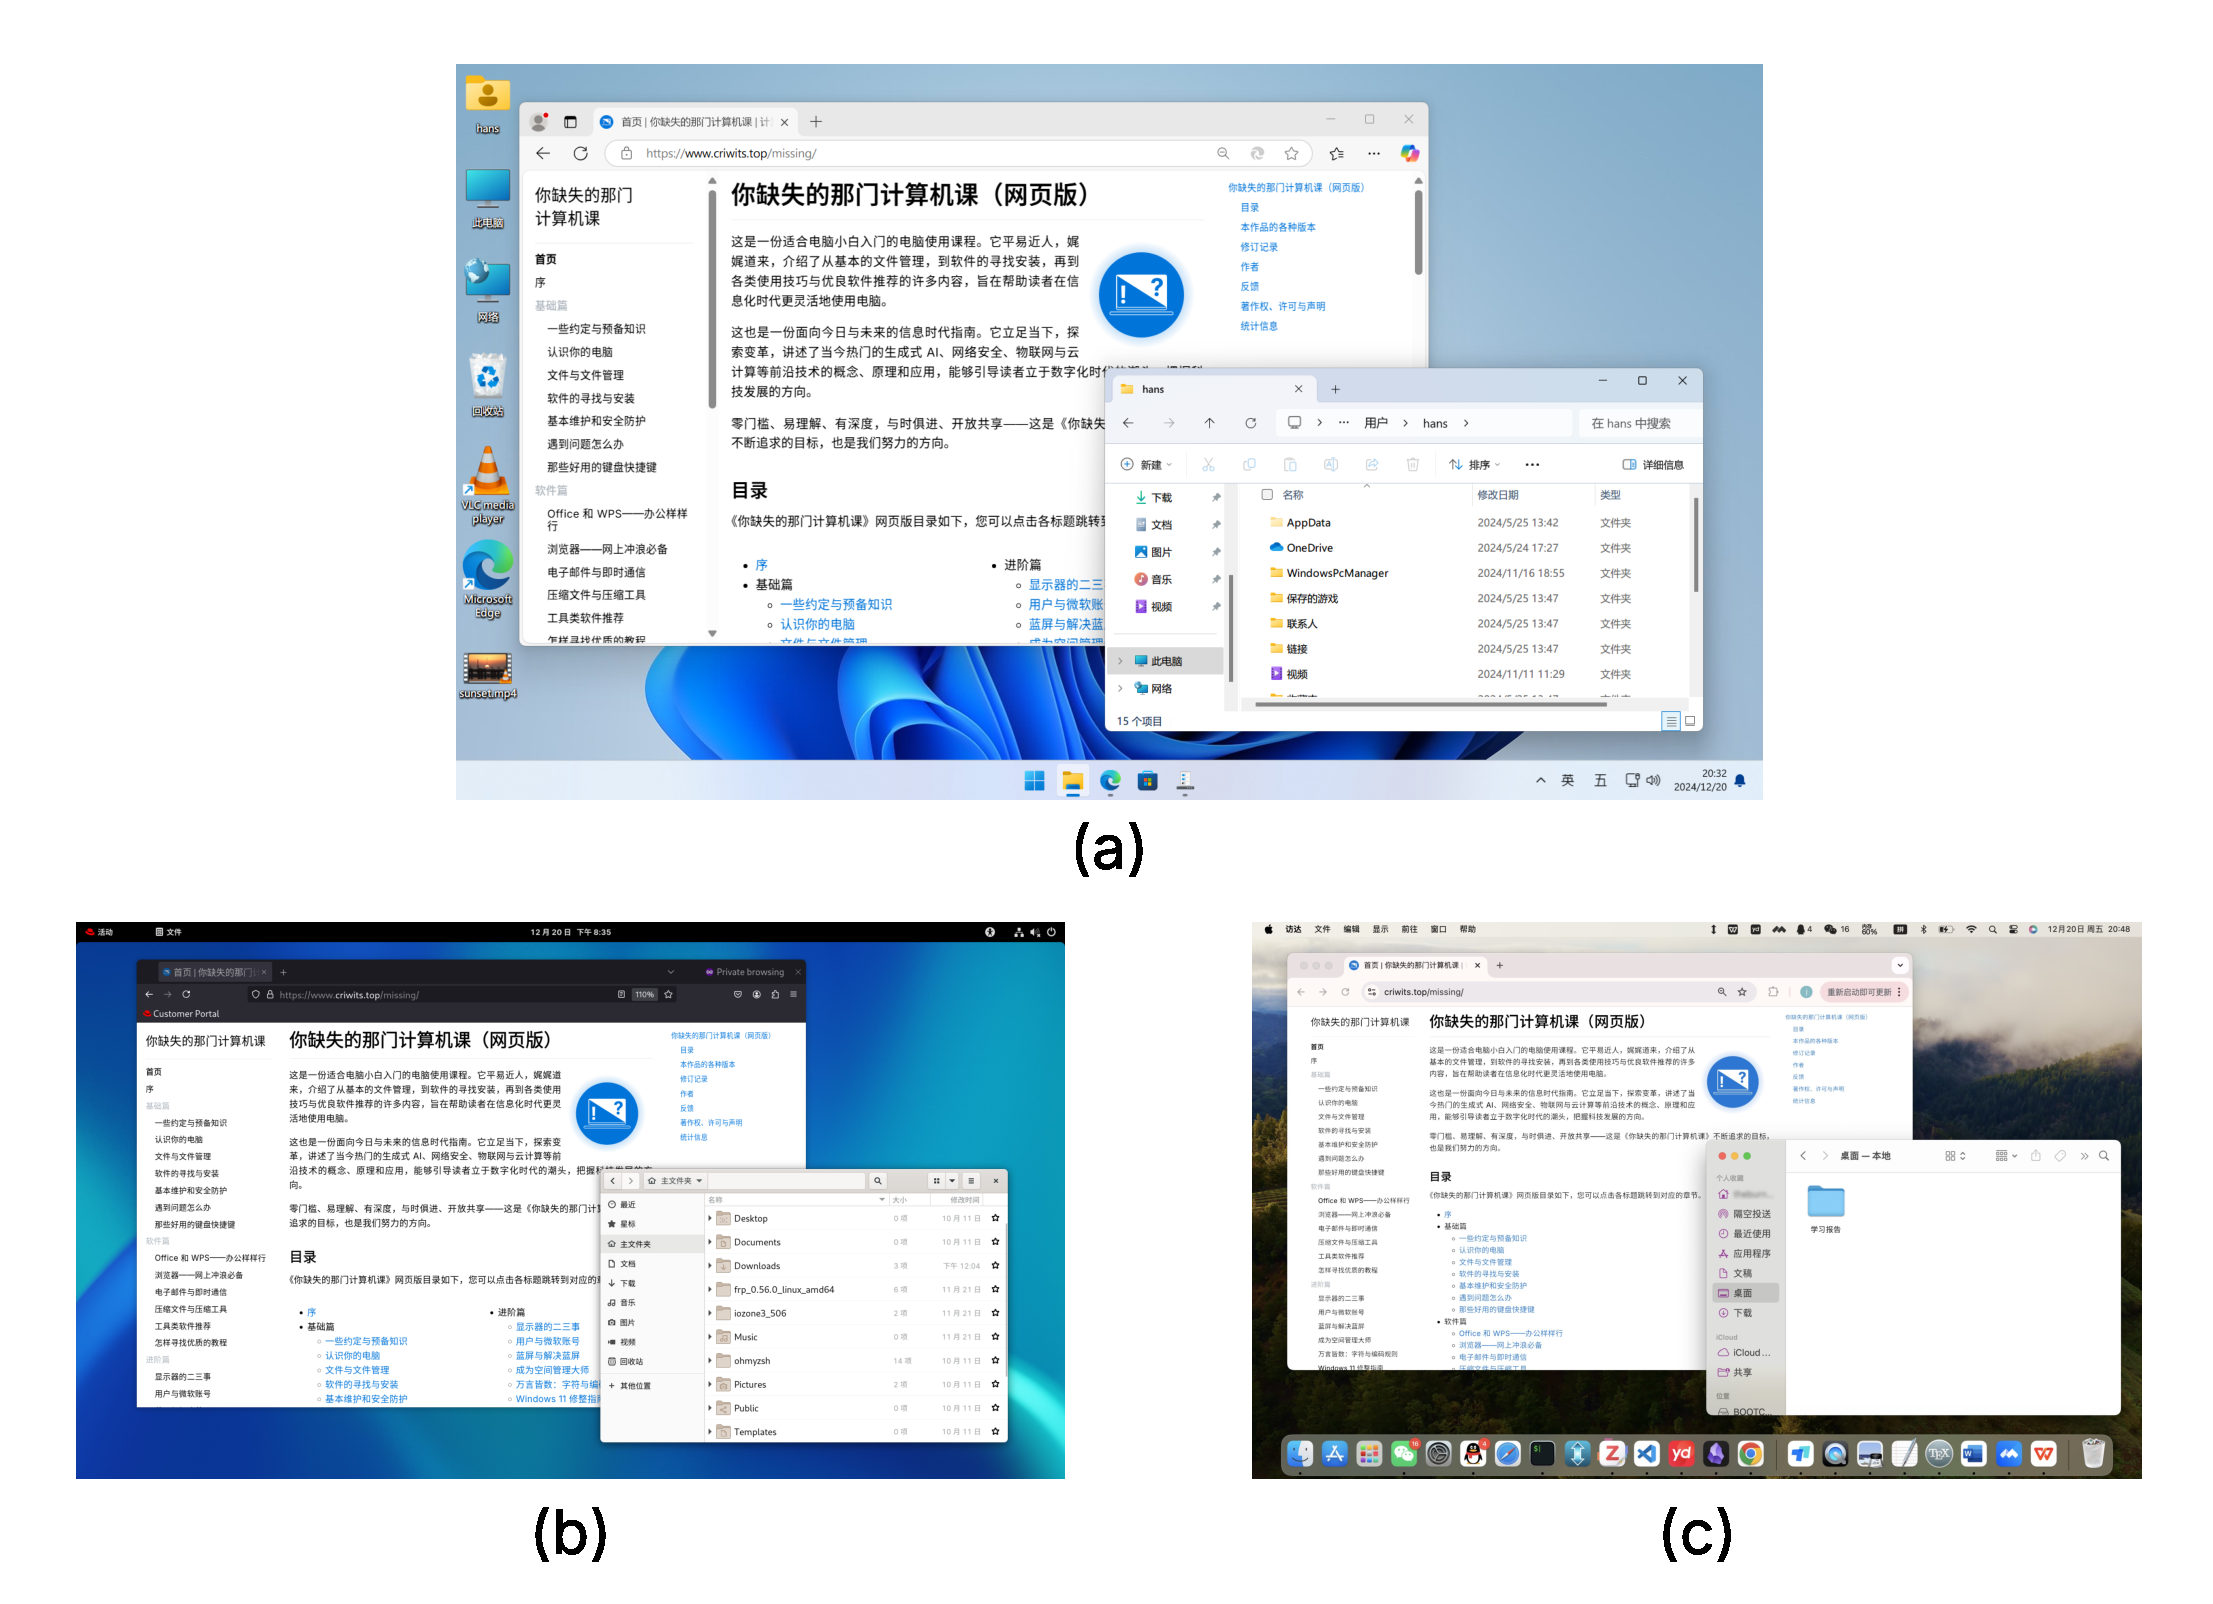
\includegraphics[width=.8\textwidth]{assets/basic/Three_systems.pdf}
  \caption{三大主流电脑操作系统}
  \label{fig:Three_systems}
\end{figure}

\subsection{Windows 操作系统}

我们绝大多数人都在使用 Windows 操作系统,《你缺计课》亦是一套基于 Windows 的电脑教程。所谓「Windows XP」「Windows 7」和「Windows 10」则是 Windows 操作系统的不同版本。

Windows 由美国的微软公司所开发,诞生于 1985 年。到今天(2024 年),Windows 已经经历了数个大版本的更新\footnote{关于 Windows 的一点点更新历史,可以参见“\nameref{cha:recover-from-bsod}”一章。}。今天,除了苹果以外几乎所有品牌的个人电脑都运行着 Windows 系统。目前最新的 Windows 版本是 Windows 11(发布于 2021 年 10 月 5 日),它与 Windows 10(发布于 2015 年 7 月 29 日)一同占领了大部分电脑。在有些地方,一些稍旧的计算机运行着 Windows 7,而更老的 Windows 版本(如 Windows XP)目前已经鲜有使用。不同版本 Windows 系统之间会有操作细节、使用体验上的不同,不过往往最直观的不同是它们的外观。下图中,(a) 和 (b) 分别展示了 Windows 11 和 Windows 10 的界面。

\begin{figure}[htb!]
  \centering
  \includegraphics[width=.9\textwidth]{assets/basic/Win_11_and_10.pdf}
  \caption{如今的两大Windows}
  \label{fig:Win_11_and_10}
\end{figure}

通过右键桌面上的【此电脑】并点选【属性】,或打开系统设置,选择【系统】→【系统信息】(Windows 10 则是【关于】),你可以看到自己电脑 Windows 系统的版本。

\begin{figure}[htb!]
  \centering
  \includegraphics[width=.7\textwidth]{assets/basic/Check_Windows_version.png}
  \caption{检查 Windows 系统版本}
  \label{fig:check-windows-version}
\end{figure}

\regcolor{本书假定读者使用的系统是 Windows 11 或者 Windows 10,其中所有的操作都是基于 Windows 11 或者 Windows 10 简体中文版系统来描述的。}不过,本书所介绍的知识是通用的,如果你使用的是 Windows 7、Windows 8 或者 Windows 8.1,本书提到的多数操作你也能正常使用。一些明确仅能用于 Windows 10 和/或 Windows 11 的操作和技巧一般会特别标注。

\practice

\begin{enumerate}
  \item 通过任务管理器和【此电脑】→【属性】,查看自己电脑的 Windows 版本、CPU 型号和核心数、内存大小、硬盘大小和类型、显卡大小和类型。
  \item 你使用的是游戏本还是轻薄本?亦或是介于二者之间的所谓「全能本」?尝试翻到笔记本的底面,上网搜索它底面所写的型号,了解关于你自己机器的更多信息。
  \item 你对「电路」的认知有多少?你是否好奇 CPU 是怎么运作的?从开关、导线、电池、灯泡组成的最简单「电路」到几乎无所不能「电脑」之间到底发生了什么奇妙的变化?在本书超越篇的\nameref{cha:program-and-arch}一章中,我们会简要向你进一步介绍这些问题。但限于《你缺计课》篇幅,我们是没法完全告诉你这些的。但是,你若有兴趣,可以去学习「电路电子技术」「计算机体系结构」「计算光刻」「纳米测量技术」等相关内容。近年来,国际形势风云变幻,我国在芯片领域仍然存在许多短板。我们希望越来越多的有志青年能投身于包括但不限于体系结构、硬件组成、数字电路乃至微电子、集成电路制造、半导体材料等领域,为我国芯片行业「补上短板」贡献自己的力量。
\end{enumerate}

\include{chapters/chap_1-2_files-and-file-management}
\chapter{软件的寻找与安装}
\label{cha:software-installation}

\begin{intro}
  都说电脑离不开软件,可是软件的寻找和安装并非易事——从哪里下?怎么下?下完怎么装?装完怎么办?什么,软件要收费?破解是什么?……这一章将对国内互联网环境下 Windows 软件的下载、安装和配置做一个简单的介绍。看完本章,你或许可以找到下面这些问题的答案,并慢慢对「怎么寻找软件」有一个初步的了解。
  \begin{itemize}
    \item 我想下载某款软件,我应该去哪里找这软件?
    \item 网上全是病毒和垃圾软件,我应该怎么样最大程度保证自己电脑的安全?
    \item 为什么软件下到手还要安装?有的还要破解?为什么这么麻烦?
    \item 电脑里不是有个「Microsoft Store」吗?为什么那里面大多数软件都找不到?
  \end{itemize}
\end{intro}

直到今天,Windows 系统下依然没有一个广泛使用的集中化「应用商店」。与我们使用手机不同,在电脑上,我们若想安装某个软件,多数情况下需要到互联网上寻找软件的「安装包」,再自行将软件安装到电脑上来使用。

这一章,我们将具体介绍如何从网上的万千垃圾软件中下载我们需要的软件,以及软件安装和配置的一些技巧和注意事项。\vspace*{-.5cm}

\section{安装与安装包}

\begin{wrapfigure}[15]{r}{5.2cm}
  \centering
  \raisebox{0pt}[\dimexpr\height-0.6\baselineskip\relax]{\includegraphics[width=5cm]{assets/basic/NCM_directory.png}}
  \caption{「网易云音乐」的目录}
  \label{fig:NCM_directory2}
\end{wrapfigure}

在 Windows 系统上,软件是通过「安装包」来安装到系统上的。如果把软件比作一棵树,那安装包就是这棵树的种子,我们需要借助安装包将软件「种」到电脑上,这个过程就是「安装」。为什么需要安装包,而不直接分发应用本身呢?解答这个问题,就有必要稍微了解一下软件在我们的电脑上的安装过程。

在上一章\chapref{cha:file-and-file-management}中我们看到,一款软件除了主程序(一个 \MissingVerb{exe} 文件)外,还包含一大堆不可或缺的依赖文件和子文件夹,如\autoref{fig:NCM_directory2} 所示。

安装包的作用之一,便是把上面这一大堆文件按照它们能够工作的结构释放到我们的电脑中的指定位置。而除了「释放文件」之外,安装包还会设置一些文件的打开方式(上一章中提到的那张「表」),并调整一些系统内部的参数。可以说,软件安装的过程,不仅仅是将一大堆文件释放或者说「提取」到系统中的某一个位置的过程,它还会对系统进行或多或少的调教与更改。这就是安装包存在的意义——它帮助我们完成了这复杂的安装过程。

\section{如何上网寻找软件的安装包}

下面我们来探讨如何上网寻找我们需要的软件的安装包。

\subsection{优先考虑:官方网站}

当要获取一款软件时,我们首先应该考虑的是它的官方网站,即「官网」。比起在其他地方下载软件,从官网下载软件能最大限度地保证你所下载的东西是干净的。

然而,\regcolor{搜索引擎中存在大量广告,且为了吸引点击量而常常放在前面,所以搜索结果中靠前的结果并不一定是官网。}例如,我们想要下载办公软件 WPS Office(简称 WPS),直接在某搜索引擎上搜索「WPS 下载」,我们会得到这样的搜索结果:

\begin{figure}[htb!]
  \centering
  \includegraphics[width=.98\textwidth]{assets/basic/Ads_in_search_engine.pdf}
  \caption{在某知名搜索引擎搜「WPS 下载」的结果}
  \label{fig:Ads_in_search_engine}
\end{figure}

如上图,我们搜索「WPS 下载」,结果中:

\begin{itemize}
  \item {\color{MissingRed} ➊ 是重庆某公司提供的广告。该公司是一个第三方的软件下载平台,我们无法确保自己能在该网站上下载到原版的 WPS。}
  \item {\color{MissingRed} ➋ 和 ➎ 是「软件中心」「下载站」类网站。与第一条一样,我们无法确保其能够提供原版软件,也难以确保其不会捆绑安装我们不需要的软件。}
  \item {\color{MissingRed} ➌ 是成都某公司提供的广告。首先它提供的产品并非 WPS 而是「Office」,其次该平台出售的 Office 软件是否取得微软官方的正版授权也值得商榷。}
  \item {\color{MissingGreen} ➍ 才是 WPS 的官网。注意看它的网址以 \MissingTT{.wps.cn} 结尾,这是 WPS 的官方网站。}
\end{itemize}

鉴别一个网站到底是不是官网,我们主要可以观察这么几个地方:

\begin{itemize}
  \item 看网址。一般官网的网址都是企业或者软件的名字。例如:
  \begin{itemize}
    \item WPS 的官网是 \texttt{wps.cn}。
    \item QQ 的官网是 \texttt{qq.com}。
    \item 网易云音乐的官网是 \texttt{163.com}。
    \item Steam 的官网是 \texttt{steampowered.com}\footnote{如果你想快速去到 Steam 的官网,可以直接访问 \href{https://s.team}{\texttt{s.team}}。}。
    \item ……
  \end{itemize}
  \item 排除法。没有哪个软件厂商的名字是叫做「✕✕软件站」「✕✕下载站」「✕✕软件园」的。带有这些名字的\textbf{全部}是第三方下载站。
  \item 语义判断。一般广告网站的标题都与搜索关键词没有任何实质上的联系。我们不妨再看上面的搜索结果中的前几条广告,会发现它们通常名不副实(如「办公软件」「Office」而非「WPS」)。
\end{itemize}

当我们下载的软件是国外软件时,这一问题会变得更加严重。假设我们想下载国外著名游戏平台 Steam 的客户端,我们在搜索引擎上搜索「Steam 下载」,得到的结果如下:

\begin{figure}[htb!]
  \centering
  \includegraphics[width=.98\textwidth]{assets/basic/Ads_in_search_engine_2.pdf}
  \caption{在某知名搜索引擎搜「Steam 下载」的结果}
  \label{fig:Ads_in_search_engine_2}
\end{figure}

作为一款国外平台,图中 ➊、➋、➍ 和 ➐ 的由国内公司提供的内容显然都不可能是官网。而对于 ➌ 和 ➎,虽然它们看起来好像是 Steam 官方网站,但请注意它们的介绍中都含有「手机版」字样,而 Steam 是用来购买电脑游戏的平台(不过 Steam 确实有手机版,用于在手机上浏览和购买游戏等),同时这两个结果的域名也并非 Steam 官方的 \texttt{steampowered.com}。事实上,只有 ➏ 所对应的 \url{store.steampowered.com} 网址,才是 Steam 真正的官网。

再以著名的开源录屏与直播软件 OBS Studio(简称 OBS)为例。我们搜索「OBS 下载」,会得到类似\autoref{fig:Ads_in_search_engine_3} 的搜索结果。

\begin{figure}[htb!]
  \centering
  \includegraphics[width=.98\textwidth]{assets/basic/Ads_in_search_engine_3.pdf}
  \caption{在某知名搜索引擎搜「OBS 下载」的结果}
  \label{fig:Ads_in_search_engine_3}
\end{figure}

根据内容提供方的名称,我们很容易可以排除 ➊、➋、➌、➍ 和 ➐ 这些国内公司提供的广告。至于 ➑,注意它的域名以 \MissingTT{.cn} 结尾——这是我国的顶级域名,自然不会被 OBS 这样一个国外开源软件的官网所用。➒ 的网站名称为「✕✕下载」,说明该网站是一个「下载站」而不是软件的官网。实际上,OBS 的官网域名是 \texttt{obsproject.com},搜索结果中 ➏ 和 ➐ 两项为官网。

进入软件的官方网站之后,我们搜索「全部产品」「软件下载」之类的选项,就可以找到我们所需要的软件的安装包。对于那些支持多种不同操作系统的软件,\regcolor{我们需要选择包含「Windows」或「Win」字样,或扩展名为 \MissingTT{exe} 的选项}。如果软件还有「32 位」「64 位」,或者「32-bit」「64-bit」以及「x86」「x64」之分,我们还需要查看自己操作系统的类型。打开系统设置,选择【系统】→【系统信息】(Windows 10 则是【关于】),在【设备规格】下找到【系统类型】一栏,然后根据下表选择合适的下载项。

\begin{table}[htb!]
  \centering
  \caption{选择合适的下载项}
  \label{tab:choose_arch}
  \begin{tblr}{
    colspec = X[.9]XX[1.6],
    cells = {j, m},
    row{1} = {halign=c, fg = white, bg = missing, font = \bfseries},
    row{even} = {MissingSkyBlue},
  }
    \toprule
    系统类型 & 建议选择 & 备注 \\
    \midrule
    32 位操作系统, 基于 x86 的处理器 & 32 位软件(32-bit、x86、i386、win32) & 只能下载 32 位软件 \\
    32 位操作系统, 基于 x64 的处理器 & 32 位软件(32-bit、x86、i386、win32) & 只能下载 32 位软件 \\
    64 位操作系统, 基于 x64 的处理器 & 64 位软件(64-bit、x64、x86-64、amd64、win64) & 优先下载 64 位软件,但 32 位软件亦可使用 \\
    64 位操作系统, 基于 ARM64 的处理器 & ARM 64 位软件(arm64、aarch64) & 此类 CPU 比较特殊\footnotemark,优先下载含有 ARM 字样的软件,若无,则尝试使用 64 位软件,若无法使用则再尝试 32 位软件 \\
    \bottomrule
  \end{tblr}
\end{table}
\footnotetext{有关这些的具体细节,请参见本书超越篇的\chapref{cha:program-and-arch}一章。}

\begin{note}
  一些软件可能有「安装版」和「便携版」之分——前者像普通软件一样,需要安装使用,而后者不必安装,下载后可以直接运行(可能需要解压)。一般来说,安装版文件名含有「setup」字样,而便携版可能有「portable」字样。一般我们建议下载安装版。
\end{note}

例如,在 WPS 官网下载 WPS 软件:

\begin{figure}[htb!]
  \centering
  \includegraphics[width=10cm]{assets/basic/Download_WPS.png}
  \caption{从官网下载 WPS}
  \label{fig:Download_WPS}
\end{figure}

或是在 OBS Studio 官网下载 OBS Studio 软件:

\begin{figure}[htb!]
  \centering
  \includegraphics[width=10cm]{assets/basic/OBS.png}
  \caption{从官网下载 OBS Studio}
  \label{fig:OBS}
\end{figure}

\subsection{直面深渊:第三方软件站}

\begin{note}
  2022 年央视「3·15 晚会」对一些软件下载站的捆绑下载行为进行了曝光\footnotemark。在被曝光之后,各大下载站均紧急撤下了「高速下载」这样的诱导性下载按钮。目前,在这些第三方下载站上,带有诱导性质的「安全下载」按钮仍然存在,不过会标明「需通过✕✕下载」。
\end{note}
\footnotetext{详见 \url{https://www.bilibili.com/video/BV1JZ4y167m8}。}

在某些时候,我们确实找不到一个软件的官网,或者因为这样那样的原因不能去官网下载某个软件。这时,我们将不得不直面深渊,进入各种各样的第三方下载站下载软件。

实际上,在这些网站上,我们一般是可以下载到想要的东西的——前提是,你足够小心,不点到那些所谓「高速下载器」「P2P 下载器」的虚假链接,也不点击到任何诱导下载的广告。下面我们会手把手实操这个过程。

假设我们要下载「OBS Studio」这款软件。我们在网上搜索「OBS 下载」,并主动避开那些广告,找到了这个名为「✕✕之家」的第三方软件站:

\begin{figure}[htb!]
  \centering
  \includegraphics[width=.7\textwidth]{assets/basic/OBS_third_party.png}
  \caption{「✕✕之家」上的 OBS Studio}
  \label{fig:OBS_third_party}
\end{figure}

重点来了:进入这个网站后,\regcolor{请避开所有【高速下载】【极速下载】【安全下载】【P2P 下载】这样的按钮},并且不要点击任何广告。相反地,我们选择【普通下载】【本地下载】这样的按钮:

\begin{figure}[htb!]
  \centering
  \includegraphics[width=10.5cm]{assets/basic/Download_page_1.png}
  \caption{不要选择【安全下载】,选择【本地下载】}
  \label{fig:Download_page_1}
\end{figure}

点击之后我们会跳转到这样一个「下载地址」的页面。同样地,我们不要点击「优先使用✕✕管家下载」之下的所有链接,而要点击「普通下载地址」下方的【通用网络下载】等链接:

\begin{figure}[htb!]
  \centering
  \includegraphics[width=10.5cm]{assets/basic/Download_page_2.png}
  \caption{选择「普通下载地址」中的链接}
  \label{fig:Download_page_2}
\end{figure}

我们使用【通用网络下载】得到的文件是一个体积约 133 MB 的压缩包,如\autoref{fig:Real_OBS} 所示,符合这个软件的体量。将这个压缩包解压,我们就能得到 OBS Studio 的安装包。而使用上方所谓【安全下载】下载到的文件如\autoref{fig:Fake_OBS} 所示,体积只有 20.3 MB,而且是一个不明的「可执行文件」(\MissingTT{exe} 文件)。与前面相比,这个文件就显得很可疑了。事实上,它不是 OBS Studio 的安装包,而是一个名不见经传的「✕✕管家」的安装包。这个「管家」可能会恶意地给我们的电脑安装许多来历不明的软件。

\begin{figure}[htb!]
  \centering
  \begin{minipage}{.48\textwidth}
    \centering
    \includegraphics[width=.8\textwidth]{assets/basic/Real_OBS.png}
    \caption{真的 OBS 安装包}
    \label{fig:Real_OBS}
  \end{minipage}
  \begin{minipage}{.48\textwidth}
    \centering
    \includegraphics[width=.8\textwidth]{assets/basic/Fake_OBS.png}
    \caption{假的 OBS 安装包}
    \label{fig:Fake_OBS}
  \end{minipage} 
\end{figure}

我们用杀毒软件卡巴斯基扫描假的 OBS 安装包,结果如下:

\begin{figure}[htb!]
  \centering
  \includegraphics[width=.7\textwidth]{assets/basic/Kaspersky_app_warning.png}
  \caption{卡巴斯基的提示}
  \label{fig:Kaspersky_app_warning}
\end{figure}

而卡巴斯基提供的网页版说明,则对这种威胁有更详细的解释:

\begin{figure}[htb!]
  \centering
  \includegraphics[width=.9\textwidth]{assets/basic/Kaspersky_website_warning.png}
  \caption{卡巴斯基网站上的解释}
  \label{fig:Kaspersky_website_warning}
\end{figure}

在本章的最后,我们会向你展示这个使用【安全下载】得到的可疑文件究竟是什么。

\subsection{另辟蹊径:软件公众号及其他小众渠道}

另一种「另辟蹊径」的方法,是通过一些「小众渠道」,例如一些分享软件的微信公众号来下载软件。这不失为一种好方法——那些人们口口相传的优质公众号一般会把常用软件的干净安装包分门别类地整理分享。与各种「下载站」相比,它们帮我们免去了下载到恶意软件的烦恼。

但是,这种公众号一般软件不是特别多——你总有一天没法从它们那里找到想要的软件。此外,这些公众号一般使用各种网盘平台来分享文件,而这些网盘平台通常会对非会员用户限速,这必然对使用体验有一定影响。不过总的来说,这依然是一种值得推荐的方法。

\begin{note}
  对于这类公众号,我们并没有做太多的收集,因此无法在此推荐。你可以在哔哩哔哩、贴吧、微博等网站自行寻路。
\end{note}

\subsection{他山之石:第三方的「软件管家」}

除了手动在网上——无论是在官网,从第三方下载站,还是从那些整理网站的公众号上——下载软件的安装包之外,有一些第三方的「软件管家」也能帮助我们找到所需要的软件。这些软件管家有的是电脑厂商所维护的,例如「联想软件管家」「华为软件管家」;有的是一些第三方企业所维护的,比如「360 软件管家」「腾讯软件中心」等。

一般来说,那些由电脑厂商所维护的软件管家,往往相对干净、不带「全家桶」式的捆绑;而那些第三方企业维护的软件管家,一般都会或多或少地提示用户安装它们的配套软件。比如,如果你使用 360 软件管家,那它可能就用某些手段提示用户去安装 360 安全卫士以及一系列其他软件。因此,你可以根据自身机器的实际情况,按需选择这样的软件管家类工具。

\section{安装软件}

假设经过与各种网站的斗智斗勇,你成功地下载到了某款软件的安装包。取决于软件,你下载到的可能是下面三种文件中的某一种:

\begin{itemize}
  \item 一个光秃秃的 \MissingVerb{exe} 文件或者 \MissingVerb{msi} 文件。我们直接双击这个文件就能启动安装进程。
    \begin{figure}[htb!]
      \centering
      \includegraphics[width=.6\textwidth]{assets/basic/Single_file_installer.png}
      \caption{单文件安装包}
      \label{fig:Single_file_installer}
    \end{figure}
  \item 一个压缩包,例如 \MissingVerb{zip} 或 \MissingVerb{rar} 文件。我们需要解压缩这个压缩包到某处,然后在解压出来的文件中找到「\MissingVerb{setup.exe}」「\MissingVerb{install.exe}」等名字的程序双击打开。
    \begin{figure}[htb!]
      \centering
      \includegraphics[width=.6\textwidth]{assets/basic/Archive_installer.png}
      \caption{压缩文件安装包}
      \label{fig:Archive_installer}
    \end{figure}
  \item 一个扩展名是 \MissingVerb{iso} 的文件。我们右击这个 \MissingVerb{iso} 文件,选择【打开方式】→【文件资源管理器】,然后在弹出的新窗口中找到「\MissingVerb{setup.exe}」「\MissingVerb{install.exe}」等名字的程序双击打开\footnote{当你这样打开 \MissingTT{iso} 文件后,这个文件会临时被「映射」成电脑里的一个新「分区」,打开【此电脑】就能发现它。在你安装完成后,可以打开【此电脑】,右键这个分区选择【弹出】来让这个分区消失。}。
    \begin{figure}[htb!]
      \centering
      \includegraphics[width=.6\textwidth]{assets/basic/Image_Installer.png}
      \caption{镜像文件安装包}
      \label{fig:Image_Installer}
    \end{figure}
\end{itemize}

\begin{note}
  对于那些「绿色版」或「便携版」软件,没有「安装」这一过程。要么是单单一个 \MissingVerb{exe} 文件,点开就能用;要么以压缩包形式出现,但是「开箱即用」——解压后直接运行主程序就可以用,就像下面这样。
  \begin{center}
    \includegraphics[width=.7\textwidth]{assets/basic/Portable_app.png}
    \captionof{figure}{便携版软件}
    \label{fig:Portable_app}
  \end{center}
\end{note}

启动安装器后,我们一般按提示【下一步】操作即可完成安装。但是此过程中也要留心!跨过了「高速下载器」的坎,可不要又掉进了捆绑软件的坑。\regcolor{有一些软件在安装程序中也会像「高速下载器」一样勾选了一些捆绑软件、浏览器主页等选项},这些选项可能出现在安装过程中的\regcolor{任何阶段},一定要注意取消勾选再进行下一步。

在安装过程中还需要特别注意的一件事,便是「软件安装位置」,即安装包释放软件自身各种文件的位置。

在上一章中我们提到过,如果 C 盘空间有限,就不要把大量的数据放在 C 盘。对于软件来说,同样有类似的情况:如果你的 C 盘空间本身并不大(例如,小于 300 GB),将大量的软件放在 C 盘,会使得 C 盘的空间压力随着使用时间的增长而显著增大。在这种情况下,安装到 D 盘或其他磁盘分区是更好的选择。不过,如果你的电脑总共只有一个分区(C 盘),那么直接选择安装在其中即可。

\begin{note}
  在\chapref{cha:computer-and-its-components}一章介绍硬盘时,我们说有些电脑会混合使用固态硬盘和机械硬盘。一般这种情况下,C 盘位于固态硬盘上,而后续的分区有可能位于机械硬盘上,你可以在任务管理器中查看分区和硬盘的对应关系。在这种情况下,我们建议将常用软件安装在 C 盘或者固态硬盘的分区上。
\end{note}

一般来说,软件默认会把自己释放在以下两个路径之一,它们分别是「64 位」和「32 位」软件的默认安装位置(也可能没有 \MissingVerb{<厂商名字>} 一层)。

\begin{MissingVerbatim}
C:\Program Files\<厂商名字>\<软件名字>\
C:\Program Files (x86)\<厂商名字>\<软件名字>\
\end{MissingVerbatim}

在上一章中我们提到了「快捷方式」,在你的电脑桌面上就有许多软件可执行文件的快捷方式。右键它们选择【属性】,你就能看到这些已经安装的软件的位置。看看它们中的一些是不是在 \MissingVerb{C:\Program Files\} 或者 \MissingVerb{C:\Program Files (x86)\} 下?

\begin{note}
  然而,往上面两个位于 C 盘的路径放东西是需要管理员权限的(详情可见 \chapref{cha:basic-maintenance})。而有些软件会默认把自己安装到你用户文件夹下的 \MissingVerb{AppData} 文件夹,这个文件夹默认是隐藏的,但往里面放东西不需要管理员权限。这种策略给我们管理软件安装位置带来了一些麻烦。
\end{note}

\MissingVerb{Program Files} 和 \MissingVerb{Program Files (x86)} 这两个文件夹,即系统预置的两个用来安装 app 的文件夹,都位于 C 盘根目录下。然而,我们希望把软件安装到 D 盘。这里推荐一个简单好用的方法:\regcolor{直接将默认路径中的 \MissingTT{C:} 改成 \MissingTT{D:}。}例如:

\begin{MissingVerbatim}
  D:\Program Files (x86)\Tencent\QQ\
\end{MissingVerbatim}

这就是在 D 盘安装 QQ 软件的一个很合适的路径。这样做能保持一个比较干净的目录结构。你的 D 盘下会因此多出 \MissingVerb{Program Files} 和 \MissingVerb{Program Files (x86)} 这样的两个文件夹,用来专门在 D 盘安装软件。如下图所示,在安装软件过程中把 \MissingVerb{C} 改成 \MissingVerb{D} 即可。

\begin{figure}[htb!]
  \centering
  \includegraphics[width=7cm]{assets/basic/Change_C_to_D.png}
  \caption{快速得到 D 盘安装软件的路径}
  \label{fig:Change_C_to_D}
\end{figure}

如\autoref{fig:Sogou_change_directory} 所示,有一些软件的安装包不是「下一步」型的,而只有一个「立即安装」的按钮。一般这种情况,可以展开「自定义安装」之类的选项,然后更改软件的安装位置。

\begin{figure}[htb!]
  \centering
  \includegraphics[width=8cm]{assets/basic/Sogou_change_directory.png}
  \caption{有时候得找「自定义安装」的选项}
  \label{fig:Sogou_change_directory}
\end{figure}

\section{软件收费、破解和自由软件}

\begin{wrapfigure}[17]{r}{6.2cm}
  \centering
  \raisebox{0pt}[\dimexpr\height-0.4\baselineskip\relax]{\includegraphics[width=6cm]{assets/basic/Adobe_PS.png}}
  \caption{Adobe 的「Creative Cloud 中国摄影计划」套装。}
  \label{fig:Adobe_PS}
\end{wrapfigure}

很多软件是需要购买的,包括 Windows 系统本身(一般你购买电脑时,电脑厂商已经帮你出了买 Windows 这部分钱)。常见的专业软件,从平面设计领域的 Adobe 家族的 Photoshop、Premiere Pro,工程领域的 Autodesk 家族的 AutoCAD、3ds MAX,到开发领域的 JetBrains 家族的 IDEA、PyCharm,甚至于我们每天都在用的 Word 和 PowerPoint,这些软件全部都需要付费购买。右图是购买正版 Photoshop(俗称的 PS)软件的页面——定价 888 元一年。

而由于这样或那样的原因,我们在实际生活中,或多或少都在「没有付费而『白嫖』这些软件」。这是因为我们使用的这些软件被「破解」了。破解之后,软件的计费功能失效,原本收费的软件通过某种方式变成了可以免费永久使用的软件。大体上,网上流传的破解软件一般有这么两种形式:

\begin{itemize}
  \item 一种是已经完全破解了的收费软件。这种软件已经经过修改,安装包往往也是民间自行制作的,可以直接走正常流程安装,安装后打开就可以无限制地使用。例如一些破解版的 Adobe 软件套装。
\end{itemize}

\begin{itemize}
  \item 另一种是使用收费软件的试用版本安装软件,再外加「破解补丁」。这种软件的安装包依然是使用官方原版的安装包,安装完成之后,通过某种「打补丁」的方式来外挂、欺骗这官方原版的软件,让原版软件以为用户已经购买,从而解锁全部的功能并让用户无限制使用。常见的 Office 软件的破解、Autodesk 软件的破解都属于此类。
\end{itemize}

使用破解软件终究是一件上不得台面的事情。一般来说,如果你使用破解软件作为私下的个人使用、学习,软件厂商有可能不会进行追究。\regcolor{但是,如果你将破解软件(或者说,盗版软件)用于商业用途,那必然迟早会受到追究。}尽管实际生活中软件厂商维权的积极程度各有差异,尽管我们可能会因为各种各样的原因不得不去使用破解软件,但我们仍然呼吁大家支持正版软件,万不得已使用盗版、破解软件时,仅作为非商业的个人和学习用途。

与那些用来盈利的商业软件不同,「自由与开源软件」(Free and Open Source Software,简称 FOSS)不仅是免费的,而且还允许用户在一定条款之下自由地共享、分发,甚至是修改它们的源代码,来基于它们创造出新的软件。这使得自由和开源软件能够集思广益,实现「众人拾材火焰高」:软件的发展离不开社区的贡献,而社区又随着软件的发展而更加壮大。近些年来,自由和开源软件作为一种新浪潮,在越来越多的领域开始出现,并开始动摇过去一些不可或缺的商业软件的地位。

\regcolor{《你缺失的那门计算机课》相信自由与开源软件的力量,始终支持它们的发展。}在本书的创作过程中,我们就使用了大量的自由与开源软件来进行内容创作,如使用 \href{https://inkscape.org/}{Inkscape} 绘制所有示意图,以及使用 \href{https://www.gimp.org/}{GIMP} 处理原始照片。我们鼓励大家在实际使用电脑的过程中,多多尝试、使用一些优质自由与开源软件。在本书的后续章节中,我们会推荐一批各个领域的优质软件,其中就有许多自由与开源软件的身影。

\section{UWP 应用和 Microsoft Store}

微软早在多年前就意识到,Windows 系统下一直缺少一个官方维护的、像苹果的 App Store 那样集中化的软件中心,用户下载软件只能像上文那样上网去苦苦找寻。彼时的微软公司正打算进军手机行业,想要和安卓与 iOS 形成三足鼎立之势。微软于是心想:不如弄一种新的软件格式,让软件不仅能在我们的 Windows 电脑上运行,还可以在手机上运行;然后再顺带弄一个全是这种新格式软件的应用商店,可谓一举两得。于是微软就这么干了:这种新格式叫做「通用 Windows 平台应用」(Universal Windows Platform app,简称「UWP 应用」),这个应用商店就是我们电脑里的「Microsoft Store」:

\begin{figure}[htb!]
  \centering
  \includegraphics[width=.7\textwidth]{assets/basic/Microsoft_Store.png}
  \caption{开始菜单里的 Microsoft Store}
  \label{fig:Microsoft_Store}
\end{figure}

可是,时过境迁:微软终究没有能在手机市场打下一片江山,微软做的手机系统最终在 2020 年完全谢幕。或许是微软心想,这「UWP 应用」的先进构想和 Microsoft Store 不能开了头就没了尾,因此它们直到今天依然被保留在 Windows 系统之中。

如果你有打开过 Microsoft Store,你会发现,其中有一些应用是我们日常生活中的常用应用,而另外的大多数应用,我们都从来没有听说过。而事实上,如果你去仔细查看那里面的常用应用,会发现它们往往更新得没有官网勤快,有些甚至已经停止了更新。

\begin{figure}[htb!]
  \centering
  \includegraphics[width=.75\textwidth]{assets/basic/Software_in_MS_Store.png}
  \caption{Microsoft Store 里的软件}
  \label{fig:Software_in_MS_Store}
\end{figure}

事实上,这就是 Microsoft Store 的现状:作为推广「UWP 应用」的第一线,它没有什么很拿得出手的杀手锏;作为各种「软件中心」的替代品,它的应用相当不全。微软在 Microsoft Store 和 UWP 应用上充满了雄心壮志,却最终落得今天的结局。

\section{演示:【安全下载】到底下载了什么}

\begin{dangerbox}
  \textbf{请不要在自己电脑上尝试运行这种来路不明的可执行程序!}
\end{dangerbox}

在上文中我们演示下载「OBS Studio」时,如果点选了【安全下载】,会得到这样一个只有 20 MB 的可执行文件:

\begin{figure}[htb!]
  \centering
  \includegraphics[width=.65\textwidth]{assets/basic/Fake_OBS_installer.png}
  \caption{假 OBS 的详细信息}
  \label{fig:Fake_OBS_installer}
\end{figure}

若是双击运行这个文件,Windows 会弹出\autoref{fig:UAC} 那样的窗口,询问【你要允许此应用对你的设备进行更改吗?】这个窗口称为「UAC 弹窗」,在下一章\chapref{cha:basic-maintenance}我们会详细介绍它。假设我们以为这个可执行文件就是 OBS Studio 的安装器,自然就放心地选择了【是】。这时,眼前自动弹出了像\autoref{fig:Fake_OBS_install} 的进度条,看似正在为我们安装 OBS Studio……

\begin{figure}[htb!]
  \centering
  \begin{minipage}{.44\textwidth}
    \centering
    \includegraphics[width=.8\textwidth]{assets/basic/UAC.png}
    \caption{UAC 弹窗}
    \label{fig:UAC}
  \end{minipage}
  \begin{minipage}{.55\textwidth}
    \centering
    \includegraphics[width=.95\textwidth]{assets/basic/Fake_OBS_install.png}
    \caption{假的 OBS 安装进度条}
    \label{fig:Fake_OBS_install}
  \end{minipage} 
\end{figure}

然而,窗口的左下角提示着我们事情并不简单。这个程序并没有为我们安装 OBS Studio;相反,它安装的是「✕✕管家」,同时还会更改我们浏览器的主页为「安全导航」。在安装进程结束后,我们的桌面上多了两样东西:一是我们通过【通用网络下载】就能得到的那个 133 MB 的真正 OBS Studio,另一个,如\autoref{fig:Unwanted_software},就是刚刚安装的\CJKsout*{图标和 Microsoft Store 神似的}「✕✕管家」。

显然,这「管家」并不是我们需要的东西,而那个 OBS Studio 真正的安装包,我们原本只需在网页上就能直接下载,经由这么折腾一通,如同「脱裤子放屁」。

\begin{figure}[htb!]
  \centering
  \begin{minipage}{.44\textwidth}
    \centering
    \includegraphics[width=.9\textwidth]{assets/basic/Unwanted_software.png}
    \caption{幽默「✕✕管家」}
    \label{fig:Unwanted_software}
  \end{minipage}
  \begin{minipage}{.55\textwidth}
    \centering
    \includegraphics[width=.95\textwidth]{assets/basic/Lightning_downloader.png}
    \caption{「光速下载器」}
    \label{fig:Lightning_downloader}
  \end{minipage} 
\end{figure}

比起脱裤子放屁,更危险的事情是:我们并不知道那些捆绑安装而来的软件,是否会继续静默地在我们不知情的情况下,继续安装更多我们不想要的软件。尽管这个「管家」经我们观测并没有在短时间内下载大量可疑软件,但在 2022 年 3 月「3·15 晚会」整治乱象之前,我们曾记录过一款在类似网站上下载到的「光速下载器」的行为。如\autoref{fig:Lightning_downloader},在它的界面上,我们可以看到右方有四个捆绑软件的复选框被默认勾选。

如果我们没有取消上面的这些勾选,那会是什么结局呢?我们在当时也作了记录。

\begin{dangerbox}
  请勿模仿!
\end{dangerbox}

\begin{figure}[htb!]
  \centering
  \begin{minipage}{.65\textwidth}
    \centering
    \includegraphics[width=.9\textwidth]{assets/basic/Computer_with_unwanted_software.png}
    \caption{被乱七八糟的软件「占领」的电脑桌面}
    \label{fig:Computer_with_unwanted_software}
  \end{minipage}
  \begin{minipage}{.34\textwidth}
    \centering
    \includegraphics[width=.9\textwidth]{assets/basic/Computer_with_unwanted_software_2.png}
    \caption{充满各种乱七八糟的软件的「开始」菜单}
    \label{fig:Computer_with_unwanted_software_2}
  \end{minipage} 
\end{figure}

如\autoref{fig:Computer_with_unwanted_software} 和\autoref{fig:Computer_with_unwanted_software_2} 那样,可以看到电脑已经被乱七八糟的软件占领。

虽然在那场「3·15 晚会」过后,诸多软件站的行为已经变得收敛许多,在上面的例子中所展示的【安全下载】,看似也仅仅是捆绑安装了一款「✕✕管家」。不过,这并不代表着我们就可以放松警惕——在互联网的世界中,我们永远是自己的第一安全责任人。

\practice

\begin{enumerate}
  \item 在\autoref{fig:How_to_1} 至\autoref{fig:How_to_3} 中,怎样操作最不可能下载到垃圾?
  \begin{figure}[htb!]
    \centering
    \begin{minipage}{.6\textwidth}
      \centering
      \includegraphics[width=.9\textwidth]{assets/basic/How_to_1.jpg}
      \caption{下载「谷歌浏览器」}
      \label{fig:How_to_1}
    \end{minipage}
    \begin{minipage}{.39\textwidth}
      \centering
      \includegraphics[width=.8\textwidth]{assets/basic/How_to_2.jpg}
      \caption{下载「QQ」}
      \label{fig:How_to_2}
    \end{minipage}
  \end{figure} 
  \begin{figure}[htb!]
    \centering
    \includegraphics[width=.6\textwidth]{assets/basic/How_to_3.jpg}
    \caption{下载「WPS」}
    \label{fig:How_to_3}
  \end{figure}
  \item \autoref{fig:How_to_4} 的界面中有几个捆绑勾选?
  \begin{figure}[htbp]
    \centering
    \includegraphics[width=8cm]{assets/basic/How_to_4.jpg}
    \caption{下载「微信电脑版」时不慎下载到的「高速下载器」}
    \label{fig:How_to_4}
  \end{figure}
  \item 下载「微信电脑版」,下面三个文件体积中哪一个最可能不是垃圾软件?
  \begin{enumerate}
    \item 640 KB
    \item 1.1 MB
    \item 150 MB
  \end{enumerate}
  \item 下面四个软件安装路径,谁最合适?其他的不合适在哪里?
  \begin{enumerate}
    \item 安装 Steam:\MissingVerb{C:\Program Files\steam}
    \item 安装微信电脑版:\MissingVerb{D:\Program Files (x86)\Tencent\Wechat}
    \item 安装 Vivado:\MissingVerb{D:\软件\Xilinx\Vivado}
    \item 安装网易云音乐:\MissingVerb{桌面\我的软件\Cloudmusic}
  \end{enumerate}
  \item 假设某个软件已经被安装在了一个地方,我现在想把这个软件放到另一个地方,可以直接剪切移动整个软件的目录到另一个地方吗?
  \item 查看自己电脑上 5 个不同软件的安装位置,并打开它们的安装目录,看一看里面的结构。
\end{enumerate}
\chapter{基本维护和安全防护}
\label{basic-maintenance}

\begin{intro}
  上一章我们认识到了「网络世界的险恶」——各种垃圾软件层出不穷、安装捆绑无处不在。
  在这样的环境之下,掌握电脑的简单维护方法显得尤为重要。阅读完这部分内容,你将找到下面这些问题的答案:
  \begin{itemize}
    \item 不小心安装了不想要的软件,怎么卸载它们?
    \item 为什么打开有些 app 时,系统总是提示「是否运行此应用对你的电脑进行更改」?
    \item 杀毒软件?安全中心?电脑管家?到底用什么?
    \item 为什么电脑天天都在「更新」?
    \item 网络上不干净的东西这么多,我要怎么才能「洁身自好」?
  \end{itemize}
\end{intro}

掌握一定的电脑维护的方法,例如软件的卸载、流氓软件的排查,以及了解一些电脑的安全维护的策略和措施是保障我们「网上冲浪」安全的重要一环。
在这一部分,我们将了解一些常用的电脑维护技巧,以及一些电脑安全方面的常识。

\section{软件的卸载}

上一章我们介绍了软件的寻找与安装,这里我们介绍软件的卸载。
软件的安装需要通过安装包来进行,而软件的卸载则是安装的逆过程,除了删除软件自身的文件之外,还会撤销一些写入系统的修改,解除一些文件关联等。
因此,软件的卸载也需要通过软件自身提供的卸载工具进行,而不是直接「删除」了事。

在 Windows 10 系统上,一般的软件卸载可以按下面的步骤进行:

\begin{itemize}
  \item 打开系统【设置】。
  \item 选择【应用】:
    \begin{figure}[htb!]
      \centering
      \includegraphics[width=6cm]{assets/Win_10_Apps.png}
      \caption{Windows 10 设置中的【应用】}
      \label{Win_10_Apps}
    \end{figure}
  \item 稍等片刻以使得列表完全加载。在这个界面上,会列出电脑中安装的所有软件。找到我们不想要的软件,然后点击两次【卸载】:
    \begin{figure}[thb!]
      \centering
      \includegraphics[width=11cm]{assets/Win_10_Uninstall.png}
      \caption{在 Windows 10 中卸载应用}
      \label{Win_10_Uninstall}
    \end{figure}
  \item 根据提示进行卸载操作即可。
\end{itemize}

而在 Windows 11 上则是这样:

\begin{itemize}
  \item 打开系统【设置】。
  \item 如图 \ref{Win_11_Apps},在界面左侧点击【应用】。
    \begin{figure}[htb!]
      \centering
      \begin{minipage}{6.5cm}
        \centering
        \includegraphics[width=6cm]{assets/Win_11_Apps.jpg}
        \caption{Windows 11 设置中的【应用】}
        \label{Win_11_Apps}
      \end{minipage}
      \quad
      \begin{minipage}{7cm}
        \centering
        \includegraphics[width=6cm]{assets/Win_11_Apps_and_Functions.jpg}
        \caption{Windows 11 设置中的【应用和功能】}
        \label{Win_11_Apps_and_Functions}
      \end{minipage}
    \end{figure}
  \item 如图 \ref{Win_11_Apps_and_Functions},再在右侧点击【应用和功能】。
  \item 等待右侧下方的列表加载完成。这个列表就是你的电脑上安装的所有软件。找到你不想要的软件,点击这一行右侧的【\makebox[.8em]{⁝}】,再点击【卸载】:
    \begin{figure}[htb!]
      \centering
      \includegraphics[width=13cm]{assets/Win_11_Unistall.jpg}
      \caption{在 Windows 11 中卸载应用}
      \label{Win_11_Unistall}
    \end{figure}
  \item 之后根据提示卸载即可。
\end{itemize}

一般来说,卸载很快就能完成。但需要特别注意的是,\regcolor{一些国产软件的卸载界面错综复杂,充斥有大量的无关选项(例如「再想想」「我要重装」等长得巨大却又不是继续卸载的按钮),因此在点选时务必十分小心。甚至有些国产软件在卸载完成后会诱导用户装一个新的其他软件,请千万注意。}
就如图 \ref{Confusing_Uninstall} 一样。

\begin{figure}[htb!]
  \centering
  \includegraphics[width=8cm]{assets/Confusing_Uninstall.png}
  \caption{赤裸裸的诱导安装}
  \label{Confusing_Uninstall}
\end{figure}

卸载完成之后,可能需要重启电脑使得卸载完全进行。

\section{应用的权限与 UAC 弹窗}

这一节我们简单介绍 Windows 系统中的权限机制\footnote{如果你在使用中压根没见过如图 \ref{UAC} 一样的窗口(即 UAC 弹窗),那么这一整节的内容对你可能不适用。}。
在 Windows 系统中,一个程序(「可执行文件」,或者说 app)在一开始启动时仅被赋予了有限的「权限」——它不能更改系统的一些关键设置,不能在系统中安装新的软件,不可以动一些关键数据。
对于大多数程序来说,这有限的权限够用了:一般 app 也不会去动那些系统级的设置或者给你装一个什么新软件。
它们只需要「安分守己」地读写自己的文件,帮助用户完成工作就可以了。

但是,在一些特殊的情况下,这种有限的权限对程序来说会变得不够用。例如:

\begin{itemize}
  \item 对于\regcolor{安装包}来说,安装包本身的工作就是安装新的软件,而有限的权限禁止了这种行为。
  \item 对于一些\regcolor{专业软件}来说,它需要连接到一些系统级的部件才能工作,而有限的权限禁止了这种行为。
  \item 对于一些\regcolor{「系统优化」类的软件}来说,它本身就是需要更改系统设置的,而有限的权限禁止了这种行为。
\end{itemize}

\begin{wrapfigure}{r}{6.5cm}
  \centering
  \includegraphics[width=6cm]{assets/UAC.png}
  \caption{一个 UAC 弹窗}
  \label{UAC}
\end{wrapfigure}

此时,程序需要「提升自己的权限」来完成自己的工作,这个过程称为「提权」。
而下面展示的这种弹窗(「你要允许此应用对你的设备进行更改吗」,称为「UAC 弹窗」),则是程序在向系统申请「提权」时,系统对用户的提示。
这样就能解释,为什么在大多数安装或者卸载软件的时候,系统都会弹出这个窗口询问我们;而只有我们点击【是】,安装或者卸载才能正常继续了。

那么这种「UAC 弹窗」的意义是什么呢?
想象一下这个场景:你电脑上的某个垃圾软件留下的「种子」正在蠢蠢欲动,想要给你电脑安装一套流氓软件。
然而,在一开始,这枚「种子」是没有足够权限的,因此它邪恶的计划就这样直接被粉碎了——没有提升的权限,它就没有办法进行软件安装。
这也告诉了我们一个重要的事实:\regcolor{如果电脑没有操作就弹出了不明的「UAC 弹窗」,请一律拒绝。}

一般来说,「提权」这件事是软件自行向系统申请的。
但是有一些软件设计时考虑不周全,它不会自行向系统申请「提权」,但它正常工作又必须有提升的权限。
对于这样的软件,我们可以在启动它时点击右键,选择【以管理员身份运行】,在 UAC 弹窗中选择【是】,就可以手动赋予这个软件提升的权限了。
或许你会在使用中发现,一些老旧的 app 在安装时就常常需要这么做。

当然,这一套权限系统是有很多空子的。
「提升的权限」具有从属关系——如果某个 app 得到了提权,那么由它打开的其他程序也默认具有特权。
因而,如果你为一个不怀好意的 app 赋予特权,那它就可以为所欲为了——因为它能够静默地赋予其他程序特权,然后做一些不好的事情。
因而,最终我们还是需要控制住自己电脑上软件的来源,不要让「不干净」的软件来到我们的电脑上。因此,\regcolor{不运行来源不明的可执行文件},是保证安全的根本。

\section{合理使用杀毒软件和安全软件}

合理使用杀毒软件和 / 或安全软件可以保护你的电脑安全,然而不合理地使用它们,会极大地影响我们对电脑的使用体验。
这里我们会介绍一些相对「合理」的使用这类软件的方法。

首先,\regcolor{永远不要在电脑上同时安装多于一个杀毒软件}。
例如,安装了「360 安全卫士」或者「360 杀毒」,就不要再安装「火绒安全」或者「腾讯电脑管家」。
如果你同时安装多个杀毒软件,不仅没有必要,它们之间还会因权限冲突而互相「攻击」\CJKsout*{(这就是养蛊)}。

\regcolor{警惕「全家桶」}。
以「360 安全卫士」为例,它会以各种方式提示用户安装包括但不限于「360 安全浏览器」「360 极速浏览器」「360 压缩」「鲁大师」「360 游戏大厅」「360 软件管家」等一整套 360 系的产品。
而事实上,我们只是希望安装一款安全软件或杀毒软件来保护我们的电脑罢了。
稍不留神,这些软件就会因为某个勾勾没有去掉而来到我们的电脑上。

我们安装安全软件是为了保障电脑的安全,而不是希望这些软件来拖慢我们电脑的运行速度。
然而,鉴于国产软件普遍「毒瘤」的性质,合理地使用这些软件,也需要我们对它们进行「调教」。
具体地说,我们可以\regcolor{关闭那些无用的弹窗和提示},例如每次开机时恼人的「用时 xx 秒,打败全国 xx 人」的提示,桌面上碍事的「一键加速」加速球,各种「资讯」弹窗广告和「猜你喜欢」搜索框等。
这些东西与「安全」毫不相关,反而极大影响使用体验。

随着《Missing》「软件篇」的更新,我们将会推荐一些相对优秀的杀毒软件和安全软件。

\section{Windows 更新——让人又爱又恨的「更新」}

Windows 一直在不断的更新之中——这里的「更新」指的不是诸如「Windows 7」「Windows 10」这样的大版本的更新,而是那时不时阻碍我们关机睡觉的「Windows 更新」。
打开电脑的【设置】,Windows 10 选择【更新与安全】、Windows 11 选择【Windows 更新】,你就能看到现在可用的一些 Windows 更新以及它们的状态。

\begin{figure}[htb!]
  \centering
  \includegraphics[width=13cm]{assets/Windows_Update.jpg}
  \caption{Windows 10 (左)与 Windows 11(右)的「Windows 更新」界面}
  \label{Windows_Update}
\end{figure}

在今天的 Windows 10 或者 Windows 11 系统中,Windows 更新主要会包括以下这些内容:

\begin{itemize}
  \item Windows 系统本身的补丁。其中包括一些对系统高危安全漏洞的「修补」,是微软给 Windows 中存在的安全问题的补丁。
  \item 电脑驱动程序的更新。这保证了你电脑上运行的驱动程序是最新的,(理论上)能更好地发挥电脑的性能。
  \item 电脑的「体验更新」。这是一些最直观的更新,主要包括系统外观与体验的优化。相比上面两项,这些更新更加容易被我们「感知」。
\end{itemize}

这样来看的话,Windows 更新应该是一件人见人爱的美事。
但事实并不是这样。
除了阻碍我们关机睡觉之外,Windows 更新是有一定风险的——那些第一晚跑 Windows 更新,然后第二早电脑就无法启动的「翻车」事件已是屡见不鲜。
事实上,Windows 更新和我们手机的「系统更新」本质一样,都会触碰系统最核心的部分。
如果这个过程中出了一些差错,就可能让系统损坏,轻则功能不正常,重则完全无法启动。

但我们不至于因噎废食,而且还是基本上噎不着的情况下。
事实上,上文所说的因为 Windows 更新导致系统损坏的情况,大都是因为用户在电脑更新时手动打断,而非 Windows 更新自身的问题。
Windows 更新提供了大量的系统安全补丁和更新,它们对保护系统安全的意义相当重大。
所以,仅仅为了可能因不当操作损坏电脑就禁用 Windows 更新并不理智,况且,现在完全关闭 Windows 更新的步骤也挺复杂。

因此,我们所需要做的,就是「正确」对待 Windows Update。
保证 Windows 更新的安全的最重要前提,就是\regcolor{不要打断 Windows 更新}。
事实上,在系统更新的过程中,屏幕上就会一直提示你「请不要断开电源」。
在 Windows 更新进行的过程中,我们强烈建议将电脑(包括笔记本电脑,即使它内部装有电池,即使电池是充满电的)始终连接到交流电源,同时也不要盖上笔记本的盖子,为的是让系统「不受打扰」地完成整个更新流程。

\section{远离流氓软件}

所谓流氓软件,就是指会恶意诱导用户下载、安装其他软件,「传染性」强,且难以卸载的软件。
还记得在上一章中,我们亲眼目睹了由一个不干净的「高速下载器」捆绑安装的一大群软件吗?
这个「高速下载器」就是典型的流氓软件,它所安装的这些软件中有不少更是「流氓软件」。
流氓软件具有「传染性」,即一个流氓软件可能捆绑 5 个流氓软件下来,而这 5 个则可以捆绑更多其他流氓。
最后落得的,就是一台被「玩坏了」的电脑(实验过程中,并没有任何真实电脑遭受伤害):

\begin{figure}[htb!]
  \centering
  \includegraphics[width=12cm]{assets/Computer_In_A_Mess.png}
  \caption{被「玩坏了」的电脑}
  \label{Computer_In_A_Mess}
\end{figure}

\begin{warning}
  \centering
  远离流氓软件!\par
  \large 远离流氓软件!\par
  \LARGE 远离流氓软件!\par
\end{warning}

如果你在电脑上发现了流氓软件,请卸载它们。
一般情况下,对这些软件使用正常的卸载流程是可以完成卸载的。
但\regcolor{特别注意卸载时的捆绑勾选}。
然而有些时候,部分流氓软件会出现「卸载后卷土重来」的情况,这是因为它的安装被一个上级软件控制着,使得你的电脑在联网时会自动安装流氓软件。
此时,不妨想想最近是否为一些奇怪的软件赋予了特殊权限,然后找出上级软件,优先卸载,再去卸载其他流氓软件。

下面列出了一些\regcolor{常见的流氓软件}:

\begin{itemize}
  \item 「2345」家族,包括「2345 浏览器」「2345 好压」「2345 电脑管家」「2345 看图王」等一系列软件。
  \item 「快压」「巧压」「微压」「布丁压缩」「52 好压」等一批压缩工具。
  \item 「飞速 PDF」「小树 PDF」「熊猫 PDF」「极光 PDF」等一批 PDF 查看器。
  \item 「新速头条」等资讯类弹窗软件。
  \item 「小黑记事本」等小工具类软件。
  \item 「布丁桌面」「海螺桌面」「火萤视频桌面」等「桌面」类软件。
  \item 「手机模拟大师」「Steam 游戏助手」「傲视霸主」等游戏类软件。
\end{itemize}

清单总是有限的,但流氓软件是无穷多的。
一言以蔽之,所有非你主动安装而出现在电脑上的软件,一律认定为流氓软件。
\CJKsout*{(不会吧不会吧,不会有人自己去装流氓软件吧)}

\practice

\begin{enumerate}
  \item 在图 \ref{Q_4_1} 所示的界面中,按哪个按钮可以卸载?
  \item 在图 \ref{Q_4_2} 所示的界面中,按哪个按钮可以卸载?
  \item 在图 \ref{Q_4_3} 所示的界面中,按哪个按钮可以卸载?
  \item 在图 \ref{Q_4_4} 所示的界面中,如何操作可以卸载?
    \begin{figure}[htb!]
      \centering
      \begin{minipage}{5.5cm}
        \centering
        \includegraphics[width=5cm]{assets/Q_4_1.png}
        \caption{第1题图}
        \label{Q_4_1}
      \end{minipage}
      \qquad
      \begin{minipage}{7.5cm}
        \centering
        \includegraphics[width=6.8cm]{assets/Q_4_2.png}
        \caption{第2题图}
        \label{Q_4_2}
      \end{minipage}
      \\\vspace*{2ex}
      \begin{minipage}{6.7cm}
        \centering
        \includegraphics[width=6.3cm]{assets/Q_4_3.png}
        \caption{第3题图}
        \label{Q_4_3}
      \end{minipage}
      \quad
      \begin{minipage}{6.3cm}
        \centering
        \includegraphics[width=6.2cm]{assets/Q_4_4.png}
        \caption{第4题图}
        \label{Q_4_4}
      \end{minipage}
    \end{figure}
  \item 清理电脑上的杀毒软件 / 安全软件,保留一个你用得最熟悉的。
    如果不知道哪个杀毒软件比较好,请看《Missing》软件篇。
\end{enumerate}
\chapter{遇到问题怎么办}
\label{how-to-find-solutions}

\begin{intro}
  在日常使用电脑的过程中,我们会遇到各种各样的问题。
  这里的「问题」,指的是电脑并没有按照我们的想法工作,有时还伴随着意料之外的提示语句。
  学会借助互联网等工具解决问题,是帮助我们更好地使用电脑的重要一环。
  看完这一部分,你将能找到下面这些问题的答案:
  \begin{itemize}
    \item 问题是怎么产生的?
    \item 遇到问题想找别人帮助,怎么样有效地向别人提问?
    \item 找不到人提问,怎样有效地上网查找解决方案?
  \end{itemize}
\end{intro}

软件的 bug、运行环境和方式不对、操作的不当等都会导致「问题」,都可能让我们无法正常地使用软件来完成我们的需求。
在这一部分,我们介绍「问题」和「提问」。

\section{为什么会遇到问题}

所谓遇到问题,就是指软件(包括 Windows 系统本身和系统之上的 app)没有按我们所设想的方式工作
——例如,打不开、闪退、功能不正常、特定功能无法使用、电脑蓝屏等。
遇到问题的原因是十分多样的,大体来说,可以分成以下三种:

\subsection{软件自己的问题}

不是我们的问题,而是「软件的问题」,也就是所谓的 bug。
具体来说,由于软件设计者考虑不周全,而这些考虑不周全的地方被我们给碰上了,从而产生未定义的行为,造成各种问题。

在\nameref{files-and-file-management}中我们介绍「更改用户文件夹的位置」时,我们特别强调了「千万不要把一个用户文件夹的路径设置成某个盘的根目录」。
如果不小心你这么做了,会变得非常难改回去,并且会造成一系列奇怪的后果。
这某种程度上就是 Windows 系统的问题——Windows 系统在设计的时候没有考虑到这种特殊情况,但这种情况被我们误打误撞给触发了,从而造成了一系列不可预知的结果。

\subsection{运行环境的问题}

这种情况下,软件没有问题,我们也没有问题,问题出在「在不合适的环境里运行」。
例如,某个软件 A 可能需要系统版本至少是 B 但不能太新(不能高过 C),而且需要电脑上安装了 D 和 E。
一旦这一串条件中有一个不满足,软件 A 可能就不能正常工作。

特别地,在电脑中存在一种特殊的软件,我们称它为「运行库」。
这种软件自身并没有任何实际功能,但许多别的软件需要依赖「运行库」的辅助才能工作。
如果电脑缺少运行库,很多软件就不能正常打开,而会在运行时报错。

运行库是一种「你平常感知不到,但它们非常重要」的存在。
不妨现在查看一下你电脑的应用列表(方法请参见\nameref{basic-maintenance}一章),你或许能找到名为「Microsoft Visual C++」的一个或一群软件:

\begin{figure}[htb!]
  \centering
  \includegraphics[width=10cm]{assets/VCpp_Distribution.png}
  \caption{Microsoft Visual C++ 运行库}
  \label{VCpp_Distribution}
\end{figure}

这就是「VC++」运行库。你也许会纳闷自己从来没有手动安装过它们,这是因为它们可能是在一些其他软件安装时被「顺带」安装上的。

在本章的练习中,有一题的错误产生的原因就是缺少某个运行库。

\subsection{操作不当}

这种情况下,软件没有问题,而我们操作不当。
例如,我们在进行软件设置的时候遗漏了某些关键的步骤,从而造成了问题的产生。

问题本身是多样的,产生问题的原因是复杂的,解决问题的方法也是不唯一的。
受限于篇幅和我们的精力,《Missing》是不可能在一章之中总结完所有在电脑使用过程中可能遇到的问题的。
相反,我们在这一章介绍「提问」的方法——在今天的互联网时代,我们应当动用自己的人脉和互联网,充分利用这些资源来帮助我们解决问题。而「提问」正是我们利用这些资源的手段。

\section{向他人提问的艺术}

如果我们决定就自己遇到的问题向他人提问,如何提问就成了一个值得思考的问题。
「提问」至少要让对方知道下面几件事:

\begin{itemize}
  \item 「我」遇到了什么?
  \item 「我」是如何让这种状况产生的?
  \item 「我」想要什么?
\end{itemize}

具体地:

\begin{itemize}
  \item \textbf{反映现场}。
    例如,通过截屏截取问题对应的提示。
    如果不能截屏(例如蓝屏或死机),就使用手机拍屏幕上的提示。
    截屏应该范围足够大且足够清晰,这样对方才能一次性从一张图上获取尽量多的信息——问题发生时你在做什么、软件在做什么、系统是什么情况……等。
  \item \textbf{复现操作}。
    复述问题产生的过程——「我」在哪几个操作之后导致这样的问题产生。
    问题是突然产生的,还是在「我」操作之后立即产生的?
    在问题发生之前的一段时间有没有什么值得注意的现象?
    「我」在问题发生之前干了什么?
  \item \textbf{表达需求}。
    表达自己的需求——「我」使用这个软件是要干什么?
    考虑到有些问题是软件的 bug 造成而并非我们自身的问题,通过告知被提问者我们的目的,对方可以针对性地给我们提出建议——是去解决这个问题,还是仅仅不予理会。
    毕竟很多问题并不阻碍我们工作。
\end{itemize}

当然,在请求他人帮助时应该遵循基本的社交礼仪。
这些东西我们不再赘述。

\section{上网查找问题的解决方案}

在生活中,我们自己上网搜索答案的情况远远多于向他人提问的情况。
因而,掌握如何有效地上网查找问题的解决方案,比上文讲述的提问技巧或许更加实用。

搜索引擎与提问不同,我们不能直接在百度搜索框中粘贴图片,也不能在搜索框写太多东西。
使用搜索引擎查找答案,我们需要使用「关键词」代替成段的语句来表征自己遇到的问题。
对于我们常常见到的软件出错,一般都会有一个「错误代码」以及相应的错误文本。
这个 \textbf{错误代码和错误文本就是最最重要的关键词之一}。

它可能是像图 \ref{Blue_screen_windows_10} 一样的「\verb|KERNEL_MODE_HEAP_CORRUPTION|」,
也可能是像图 \ref{Green_err_code} 一样的「\verb|0x80070490|」,
还可能是像图 \ref{3Ds_Max_err_code} 一样的「\verb|126 - 找不到指定的模块|」。

\begin{figure}[htb!]
  \centering
  \begin{minipage}{10cm}
    \centering
    \includegraphics[width=8cm]{assets/Blue_screen_windows_10.png}
    \caption{Windows 10 蓝屏}
    \label{Blue_screen_windows_10}
  \end{minipage}
  \\\vspace*{1ex}
  \begin{minipage}{6.2cm}
    \centering
    \includegraphics[width=6cm]{assets/Green_err_code.png}
    \caption{错误代码}
    \label{Green_err_code}
  \end{minipage}
  \quad
  \begin{minipage}{7.2cm}
    \centering
    \includegraphics[width=7cm]{assets/3Ds_Max_err_code.png}
    \caption{3ds MAX 错误窗口}
    \label{3Ds_Max_err_code}
  \end{minipage}
\end{figure}

\textbf{另一个重要的关键词是发生问题的软件}。
仅凭一个错误代码,你可能会找到有同一个错误代码的来自不同软件的不同问题。
因此,搜索时我们务必需要带上「什么软件发生的这个错误」。
对于蓝屏错误,软件就是「Windows 10」之类的具体版本;
对于其他软件错误,尽量用简短的语句表示具体的软件,比如「CAD 2022」「Word 2019」等。

一般来说,通过上面两个关键词一起搜索,我们已经能够通过搜索引擎定位到问题和相对应的答案了,就如图 \ref{Find_Solutions} 一样。

\begin{figure}[htb!]
  \centering
  \includegraphics[width=11cm]{assets/Find_Solutions.png}
  \caption{搜寻解决方案}
  \label{Find_Solutions}
\end{figure}

在这些教程类的文章中细细寻找,一般我们都可以解决遇到的问题。
但在多如牛毛的搜索结果中筛选我们所需要的东西,也并非一件很容易的事情。
一般来说,在搜索结果的时候我们可以注意下面几个方面:

\begin{itemize}
  \item \textbf{关注「更新时间」。}
    很多网站都会显示一篇文章是于什么时候发布的。
    当我们搜索解决问题的教程的时候,遵循「越新越好」的原则。
    例如,对于同样一类错误,一篇 2016 年的文章和一篇 2021 年的文章都给出了解决方法,那我们就优先选择 2021 年的那篇文章。
  \item \textbf{警惕洗稿文。}
    譬如「百度知道」「百度经验」以及「CSDN」这样的网站,有大量洗稿、抄袭而来的教程文章。
    这些文章最大的问题是东拼西凑,内容不完整,有些还混有不少机翻的内容。
    在寻找教程的时候,尽量不要选择这样的文章。
\end{itemize}

\practice

\begin{enumerate}
  \item 如果你准备使用「Premiere」软件制作一个视频,但在导出时弹出了下面的窗口,你应该用什么样的搜索语句上网检索?
    \begin{figure}[htb!]
      \centering
      \includegraphics[width=7cm]{assets/Q_5_1.png}
      \caption{第1题图}
      \label{Q_5_1}
    \end{figure}
  \item 如果你准备打开一个小工具程序时,弹出了这样的窗口,你应该怎么办?
    \begin{figure}[htb!]
      \centering
      \includegraphics[width=10cm]{assets/Q_5_2.png}
      \caption{第2题图}
      \label{Q_5_2}
    \end{figure}
  \item 如果你准备打开一个应用时,弹出了这样的窗口,你应该怎么办?
    \begin{figure}[H]
      \centering
      \includegraphics[width=7cm]{assets/Q_5_3.png}
      \caption{第3题图}
      \label{Q_5_3}
    \end{figure}
\end{enumerate}

\part{软件篇}

\chapter{Office 和 WPS——办公样样行}

\begin{note}
  欢迎来到《Missing》软件篇!在基础篇我们介绍了最最基本的电脑操作,例如文件管理和软件安装。
  而在软件篇中,我们会「介绍」一些软件。
  这里的「介绍」并不是教你怎么用这个软件,而是简要说明这个软件是干什么的、有什么特点,以及为什么我们会介绍它。
  请注意,《Missing》从来不是任何软件使用教程的替代品。
\end{note}

\begin{intro}
  让我们从最常见的办公软件——Office,和它的相似物 WPS,来开始我们的软件篇旅程。
  在阅读完这一部分后,你能找到下面这些问题的答案:
  \begin{itemize}
    \item 下面五个名词之间的关系:Word、PowerPoint (简称 PPT)、Excel、Office、WPS。
    \item Office 版本好多,我该选哪个?2003?2007?2019?
    \item 为什么我电脑上自带的 Office 点开之后却打开了一个网页 / 购买链接?
    \item Office 怎么装?
    \item WPS 跟 Office 有什么区别?既然前者免费,那为什么还要后者?
  \end{itemize}
\end{intro}

我们绝大多数人使用电脑,都逃不开「文档写作」「幻灯片制作」「表格处理」这么三件事。
也许你早已会用 WPS,或者 Word、PPT 以及 Excel 这些再熟悉不过的软件来做这三件事,但这些软件背后的故事或许并不为你所知晓。

仍然首先强调,这部分并不是一份 Office 软件教程。

\section{Microsoft Office}

Microsoft Office 是由微软(也就是 Windows 系统它爹)开发的办公软件套装。
称它「软件套装」,是因为 Microsoft Office 是一系列软件的组合,而非一个单个的软件。
Microsoft Office 一般被人们直接简称为「Office」。
Office 包含了一系列面向办公领域的软件。
下面列出 Office 中的一些子软件:

\begin{itemize}
  \item \textbf{Word,用于制作文稿。}
  \item \textbf{PowerPoint(往往简称「PPT」),用于制作幻灯片。}
  \item \textbf{Excel,用于制作表格和进行数据处理。}
  \item OneNote,用于记笔记。
  \item Access,用于制作和管理数据库。
  \item Publisher,用于编辑出版物(例如,成册的书籍排版)。
  \item Visio,用于绘制各种图案。
  \item ……
\end{itemize}

上面列表中的前三者,即 Word、PPT 和 Excel,是 Office 套装中人们耳熟能详的三个子应用,民间俗称「Office 三件套」。
它们三个能满足几乎所有的基本办公需求,而其他的 Office 子应用有些专业而复杂,使用的人相对不多,因而很多时候都没什么人安装。

最新版本的 Office 三件套的软件图标如下图所示。

\begin{figure}[htb!]
  \centering
  \includegraphics[width=6cm]{assets/Office_Icons.png}
  \caption{如今的 Office 图标}
  \label{Office_Icons}
\end{figure}

\subsection{Office 的历史与版本}

Office 是一款历史悠久的软件套装,它诞生于上世纪八九十年代。
近 20 年,Office 都使用年份作为版本名称。

Office 2003 是十分经典的一代 Office。
与现在的 Office 软件界面有很大不同,Office 2003 的功能按钮是一排排地「罗列」在软件界面上方的。
下图是 Word 2003 的软件界面。

\begin{figure}[htb!]
  \centering
  \includegraphics[width=11cm]{assets/Word_2003.png}
  \caption{Word 2003 的界面}
  \label{Word_2003}
\end{figure}

经典归经典,由于年代实在太过久远,在今天(2022 年),除了部分中小学的「信息技术」课堂外,我们几乎很少再见到这一版 Office。

Office 2007 同样是经典的一代 Office。
自 Office 2007 开始,Office 软件采用了一种新的用户界面——「Ribbon」。
直到今天,Office 的软件界面仍然有着 2007 版本的许多影子。
另一方面,这种新的界面与 2003 版及其之前的版本有着很大的不同。
出于这个原因,当时许多人不愿意迁移至新版本。
下图是 Word 2007 的软件界面。

\begin{figure}[htb!]
  \centering
  \includegraphics[width=11cm]{assets/Word_2007.png}
  \caption{Word 2007 的界面}
  \label{Word_2007}
\end{figure}

不难发现,Ribbon 界面的主要特点是:
功能按钮按照一定的分类分置于不同的「选项卡」中,在软件上方错落排开,与 Office 2003 那种按钮一排排罗列的操作方式大相径庭。

Office 2010 与 Office 2007 在软件界面和风格上并没有什么很大的差别。
在 2021 年以前,我国计算机二级考试 Office 科目使用的就是 Office 2010 版本,因而下面的 Word 2010 软件界面想必许多读者都不会陌生。

\begin{figure}[htb!]
  \centering
  \includegraphics[width=11cm]{assets/Word_2010.png}
  \caption{Word 2010 的界面}
  \label{Word_2010}
\end{figure}

Office 2013 开始,Office 的界面画风从原来的「拟物」变成了「扁平」,不过操作逻辑仍然是自 Office 2007 就有的那一套。
Office 2013、2016、2019 乃至 2021 在界面上长得都差不多,操作体验也差不多。
下图是 Word 2019 的软件界面。

\begin{figure}[htb!]
  \centering
  \includegraphics[width=11cm]{assets/Word_2019.png}
  \caption{Word 2019 的界面}
  \label{Word_2019}
\end{figure}

近年来,除了这种传统的「年份」Office,微软还推出了一种不断迭代更新的「Office 365」(现改名为「Microsoft 365」)。
Office 365 持续更新,不再使用年份命名,界面上与最新的 Office 版本相一致,功能上随着更新不断增加。
事实上,Office 365 在功能上与最新年份版本的 Office 并无二致,它与年份版本 Office 的最大区别在于各项「云服务」,例如文件跨设备同步等。

\begin{note}
  自 2021 年开始,我国计算机二级考试 Office 科目使用了 Office 2016 作为考试软件。
  如上文所言,Office 2013--2021 乃至 Office 365 的软件界面和操作体验都没有明显的区别,故读者在练习时若实在没有 Office 2016,可以选用其余版本作为替代。
\end{note}

\subsection{Office 的文件格式}

在 Office 2003 及以前版本中,Office 三件套使用的文件格式(扩展名)如表 \ref{Old_Office_File_Format} 所示。
自 Office 2007 开始,微软推出了一套新的 Office 文件格式——「Office 开放 XML 格式」(\href{http://officeopenxml.com/}{Office Open XML},简称「OOXML」)。
这一套格式对应的扩展名如表 \ref{OOXML_File_Format} 所示。

\begin{table}[htb!]
  \begin{minipage}{7.5cm}
    \centering\begin{tabular}{ccc}
      \toprule
      软件 & 扩展名 \\
      \midrule
      Word & \verb|doc| \\
      PPT & \verb|ppt| \\
      Excel & \verb|xls| \\
      \bottomrule
    \end{tabular}
    \caption{曾经的 Office 三件套文件格式}
    \label{Old_Office_File_Format}
  \end{minipage}
  \begin{minipage}{6cm}
    \centering\begin{tabular}{ccc}
      \toprule
      软件 & 扩展名 \\
      \midrule
      Word & \verb|docx| \\
      PPT & \verb|pptx| \\
      Excel & \verb|xlsx| \\
      \bottomrule
    \end{tabular}
    \caption{OOXML 文件格式}
    \label{OOXML_File_Format}
  \end{minipage}
\end{table}

这套新的格式尽管看起来扩展名只是多了个字母「\verb|x|」,但是与旧版格式是\textbf{完全不兼容}的。
Office 2007 以及之后的各版本,可以打开新旧两种格式的文档,并且在保存文件时可以选择保存为新旧两种格式中的某一种。
下图中,上方「Word 文档 (\textbackslash\*.docx)」便是新格式,而下方「Word 97-2003 文档 (\textbackslash\*.doc)」则是旧格式。

\begin{figure}[htb!]
  \centering
  \includegraphics[width=8cm]{assets/Word_formats.png}
  \caption{Word 的保存选项}
  \label{Word_Formats}
\end{figure}

新格式(即扩展名带「\verb|x|」的那些格式)相比旧格式支持更多的功能和排版特性。
在今天人们普遍使用 Office 2007 及以上版本的情况下,我们建议始终为自己的文档选用新格式,除非你有明确的理由去选用旧格式(现在的 Office 都是默认保存成新格式的)。

\subsection{Office 的购买和安装}

Office 是付费软件。对于 Office 365,其付费方式是「订阅制」,每年都需要付费才能使用;
对于年份版本的 Office,则采用「买断制」,一次购买便可永久使用。
同一版本的 Office(例如 Office 2019),又根据包含子应用的多少、高级功能的有无、售后服务的等级等,分为不同的档次。
例如「家庭与学生版」只包含 Word、PPT 和 Excel 三件套,没有 VBA 等高级开发功能;
「专业增强版」则包含几乎所有的 Office 功能,但售价高昂。
下图是在微软官网购买 Office 365 的产品介绍页面。

\begin{figure}[htb!]
  \centering
  \includegraphics[width=12cm]{assets/Office_365.png}
  \caption{Office 365 了解一下}
  \label{Office_365}
\end{figure}

如果需要购买 Office,可以前往\href{https://www.microsoft.com/zh-CN/microsoft-365/buy/microsoft-365}{微软官网}或者 Microsoft Store 进行购买。
如果你是大学生或大学教职工,或许你所在的学校已经为你们批量购买过正版 Office 软件。
此时,你可以通过查阅自己学校官网,或者咨询学校网络信息中心 / 正版软件服务中心来了解正版 Office 的获取方式。
图 \ref{College_Office} 是某学校正版软件平台的截图,在这里可以获取到正版的各版本 Office。

\begin{figure}[htb!]
  \centering
  \includegraphics[width=12cm]{assets/College_Office.png}
  \caption{某校提供的 Office}
  \label{College_Office}
\end{figure}

今天,许多笔记本电脑和品牌机台式机在出厂时会附赠用户一套正版 Office 软件。
这种情况下,机器首次开机后内置的 Office 软件(例如 Word 和 PPT)都是可以直接使用的。
我们只需要按照软件的提示,登录或创建一个自己的微软账号,即可完成正版验证。
不过,如果你是在电脑城组装的电脑,或者使用的非品牌零售渠道的机器,那么很可能没有这项福利。
图 \ref{JD_Office_Gift} 是在京东平台购买某笔记本电脑时的 Office 附赠提示。

\begin{figure}[htb!]
  \centering
  \includegraphics[width=7.5cm]{assets/JD_Office_Gift.png}
  \caption{买电脑送 Office}
  \label{JD_Office_Gift}
\end{figure}

Office 软件的安装方式比较简单。
取决于你获取到软件的方式,如果你是通过 Microsoft Store 购买的 Office,那么直接在 Microsoft Store 点击「安装」就可以完成 Office 软件的安装。
对于通过其他官方途径获取的 Office 安装器,大多数情况下也只需要简单地双击并按提示操作即可完成安装。

Office 这种软件自然免不了被盗版的命运。
需要注意的是,在互联网上有很多民间二次打包的「破解版」Office,这种 Office 直接安装后无需更多操作就能免费使用。
我们不建议大家使用这样的 Office——除了「盗版」本身不值得提倡外,这些二次打包的 Office 往往经过一些「精简」或者「魔改」,这可能导致少数情况下软件工作不正常甚至无法使用。
此外,这些魔改 Office 往往会有一些使用上的不便,例如每次启动时触发 UAC 弹窗(弹出窗口「你要允许此应用……」),以及文件关联莫名失效等。

\subsection{「网页版」 Office}

即使你没有购买和安装过 Office,你或许仍会发现电脑的「开始菜单」中有 Office 甚至 Word、PPT、Excel 等软件的图标,例如:

\begin{figure}[htb!]
  \centering
  \includegraphics[width=3cm]{assets/Office_Web_Icon.png}
  \caption{网页版Office的图标}
  \label{Office_Web_Icon}
\end{figure}

如果你尝试去点击这些 app,会发现打开了一个网页。
在这个页面按提示登录微软账号,最后会来到这个页面:

\begin{figure}[htb!]
  \centering
  \includegraphics[width=10cm]{assets/Office_Web.png}
  \caption{网页版Office的界面}
  \label{Office_Web}
\end{figure}

这是微软提供的免费的「网页版」Office,类似于腾讯文档或金山文档等网页产品。
点击左侧的 Word、Excel 等图标,会打开对应的网页版应用。
这些网页版的 Office 可以免费使用,但功能受限,且只有在网络良好时才能正常工作,故只能作为没有安装 Office 的应急替代品。

这个「网页版」Office 本质就是几个链接,没有软件的本体,是可以卸载的。
卸载方式可参见\nameref{basic-maintenance}。

\subsection{选择 Office 的原因}

在今天,Office 文件格式(即「\verb|doc|」、「\verb|pptx|」等文件格式)在人们的日常工作中有着绝对无可动摇的地位——绝大多数的工作资料都是通过这套格式的文件进行交换的。
Office 作为推出这套格式的本家,自然与这套格式最为契合。
因此,\textbf{选择 Office 的最主要原因,便是它对 Office 文件格式的无缝支持}。
WPS 尽管对这套格式也有着相当高的支持度,但在少数情况下,仍然会出现排版错乱、内容丢失等情况。
至于其他办公软件,大多对于 Office 文件格式的支持只能说「勉强」。

选择 Office 的另一个原因是,\textbf{Office 作为微软自家出品的软件,在 Windows 操作系统上具有相对出色的性能表现和操作体验。}
在一众办公软件中,Office 的操作手感比较舒适,且与 WPS 相比,Office 界面简洁、没有繁杂的广告和其他多余功能。
下图是在 Windows 11 系统上,Office 三件套软件的界面。

\begin{figure}[htb!]
  \centering
  \includegraphics[width=11cm]{assets/Office_on_Win_11.png}
  \caption{Windows 11 上的 Office}
  \label{Office_on_Win_11}
\end{figure}

\section{WPS}

\textbf{WPS 是除了 Office 自身外,对 Office 文件格式(包含新旧两种格式)支持最好的办公软件},可以说没有之一。
WPS 包含三个主要的子组件,分别是「WPS 文字」「WPS 演示」和「WPS 表格」,依次对标 Office 套装中的 Word、PPT 和 Excel。
WPS 使用类似于 Office 的界面,默认使用 Office 文件格式进行文件保存,因而在大多数情况下都可以作为 Office 的替代品。

\subsection{WPS 的历史}

WPS 是由\href{https://www.kingsoft.com/}{金山公司}开发的国产免费软件。
WPS 的历史最早可以追溯到 1985 年,与很多人的臆想不同,WPS 并不是靠「模仿」Office 起家的。
在那时,微软的 Office 还没有支持中文,而 WPS 作为一套独立的中文文字处理系统(word processing system, WPS),在中国市场上占有很大一席之地。
1994 年,微软的 Office 开始进入中国市场。
为了和 WPS 竞争市场,微软和金山达成协议,双方能够交叉使用对方的文件格式——这是 WPS 得以完整支持 Office 文件格式的原因。
后来,WPS 逐渐失去市场优势,于是开始走上模仿 Office 的道路,从原来的单一「文字处理系统」变成了和 Office 相仿的办公软件套装,并在操作界面上有意地向 Office 靠拢。
今天的 WPS 在办公软件的基础上,又加入了「协作办公」「云服务」等许多增值服务,建立了一整套自己的办公解决方案。

\subsection{WPS 的使用}

今天 WPS 的界面与近年新版 Office 软件的界面高度相似。
下图是 WPS 文字 2019 版本的界面截图。
对于大多数 Office 软件中的操作,WPS 中的操作方式都是相同或近似的。

\begin{figure}[htb!]
  \centering
  \includegraphics[width=10cm]{assets/WPS.png}
  \caption{WPS 文字 2019 的界面}
  \label{WPS}
\end{figure}

\subsection{选择 WPS 的理由}

WPS 对 Office 文件格式有着高度的兼容性,这意味着在绝大多数情况下 WPS 都可以作为 Office 软件的替代品。
同时,WPS 是免费软件。
这意味着,你可以在没有任何额外成本的情况下合理合法地使用它,同时获得对 Office 文件格式的最大兼容度并保持 Office 的使用习惯。

WPS 针对中国用户的使用习惯推出了一系列额外功能。
WPS 有自己的模板库,称为「稻壳儿」。
在稻壳儿中,你能找到各种各样的适合不同场景的文稿、幻灯片和表格模板,并将它们应用在自己的文档之中(可能需要额外付费)。
在一些情况下,使用这些模板能够省时省力地制作出精美的文档。
又比如,WPS 提供了自己的云服务平台(金山文档),借助金山文档能够实现多人协同编辑文件等高级功能。
下图是「稻壳儿」中提供的部分模板。

\begin{figure}[htb!]
  \centering
  \includegraphics[width=11cm]{assets/WPS_Template.png}
  \caption{「稻壳儿」模板}
  \label{WPS_Template}
\end{figure}

\practice

\begin{enumerate}
  \item 你电脑上安装有 Office 吗?你能熟练地使用它们吗?你知道你所使用的 Office 软件的版本吗?
  \item 你有使用 WPS 吗?如果有,试试探索「稻壳儿」模板商城。
  \item 前往电商平台查看一些笔记本电脑的商品详情,看看它们是否有将正版 Office 软件一并附赠。
\end{enumerate}
\chapter{浏览器——网上冲浪必备}
\label{browsers-and-how-to-choose}

\begin{intro}
  浏览器是我们浏览网页的必备工具,它们将互联网上的形形色色的网页呈现在我们面前。
  不过,各种浏览器之间的门派以及它们之间交错复杂的历史渊源,却并不为多数人所知。
  
  通过阅读完这一部分,你也许可以找到下面这些问题的答案。
  
  \begin{itemize}
    \item IE 浏览器是何方神圣?
    \item Chrome 浏览器又是何方神圣?
    \item 火狐浏览器又是何方神圣?
    \item 「360 安全浏览器」「QQ 浏览器」「2345 王牌浏览器」都是怎么来的?
    \item 我应该选择什么浏览器?
  \end{itemize}
\end{intro}

浏览器是我们「网上冲浪」必备工具。
当你访问一个网站,比如说 \url{https://missing.criwits.top/},这个网站的内容就顺着网线和 Wi-Fi 传输到了你的设备(手机或电脑或其他)上。
浏览器所做的事情,就是将这些内容按它们所设计的样子「排版」或者说「呈现」,使其能完整、正确地展现在你的屏幕上。
同时,浏览器还负责与你进行交互:假如你点了一下这个网站上的某个按钮,浏览器就要去「理解」你的点击动作,并执行相应的功能。

\begin{figure}[htb!]
  \centering
  \includegraphics[width=12cm]{assets/How_Browsers_work.png}
  \caption{浏览器干的事}
  \label{How_Browsers_work}
\end{figure}

正如做数学题有人做得快有人做得慢,「排版」同一个网页,有的浏览器排得又快又好,有的则要花费更长的时间。
浏览器之间的最直观区别,就体现在同一网络下打开网页的不同速度上。
当然,不同的浏览器也有自己的特色,有的可以帮忙屏蔽一些广告,有的可以帮你记忆各种密码,有的能与「某某电脑管家」联动来保障安全,有的则只被用来下载其他浏览器。
「IE 浏览器」「火狐浏览器」「谷歌浏览器」「360 极速浏览器」「QQ 浏览器」……
这些名字或许你早已有所耳闻,但它们究竟孰优孰劣,可能还需要深入了解才能知晓。

\section{浏览器界的「血雨腥风」}

在讨论浏览器之前,我们可以先侃一侃「浏览器战争史」。

\subsection[第一次浏览器大战——网景和微软两大巨人的单打独斗]{第一次浏览器大战{\normalsize ——网景和微软两大巨人的单打独斗}}

让我们将时间的指针拨到 30 年前。
二十世纪九十年代,互联网刚刚进入民用领域,市面上开始出现各种各样的早期网络浏览器,它们的出现拉开了一场没有硝烟的「战争」的序幕。

\begin{wrapfigure}{r}{5cm}
  \centering
  \includegraphics[width=4cm]{assets/Netscape.jpg}
  \caption{网景公司的 logo}
  \label{Netscape}
\end{wrapfigure}

这些早期网络浏览器的作者中,有一个叫马克·安德森的人比较有商业头脑——他嗅到了互联网时代的机遇。
1994 年,他和自己的伙伴成立了「网景通讯」公司,并推出了一款商业化的浏览器软件——「网景浏览器」。
网景浏览器以「共享软件」的方式运作——即软件本身需要交钱购买,但是可以先免费试用。
由于网景浏览器相比竞品(虽说那时本来也没什么竞品)更加实用、稳定,网景很快统领了浏览器的市场,并成为了互联网领域的「绝对标准」。

微软见网景在互联网领域如鱼得水赚了大钱,心里很不是滋味,于是也想在浏览器领域分一杯羹。
1995 年,微软发布了「Internet Explorer」,它简写来就是「IE」。
IE 在一开始并没有取得什么竞争上的优势——一开始,它不如网景浏览器稳定,有着更多的安全漏洞并更容易死机。
但到了 1997 年,微软发布 IE 4.0,这个版本的 IE 做了几件大事:
一是\regcolor{它变成了 Windows 系统中的一部分}\CJKsout*{(捆绑安装)},二是它终于做得比网景更好了。
自此之后,IE 迅雷不及掩耳地抢占了大量市场份额。
到了 1998 年,网景被 AOL 公司收购,原来的浏览器开发团队也解散了。

至此,微软在这一场与网景的较量之中胜出,IE 浏览器成为了浏览器界的老大,第一次浏览器大战结束。

\begin{figure}[htb!]
  \centering
  \includegraphics[width=10cm]{assets/IE_4.png}
  \caption{IE 4.0 的界面}
  \label{IE_4}
\end{figure}

\subsection[第二次浏览器大战——开放、自由的竞争与新时代的机遇]{第二次浏览器大战{\normalsize ——开放、自由的竞争与新时代的机遇}}

网景虽然在第一次浏览器大战中惨败,但它并没有立刻退出这个市场,而是希望联合更多的力量来抗衡自己的对手。
1998 年,也就是网景被收购的那年,它公开了自己的网景浏览器的源代码,成立了以 Mozilla 为名的开发社团,希望借助更多人的力量将这一股薪火传下去。

时间来到 2003 年,苟延残喘的网景公司最终解散。
解散当天,AOL 也分离了与 Mozilla 的关系,Mozilla 成为了一个独立的「基金会」。
所谓「基金会」,就是说自身不以营利为目的,而依赖社区——或者说大众——的力量进行开发,依赖用户的捐赠来维持运行。
不久后,Mozilla 将自己开发的,「传承」自网景的浏览器赋予「Firefox」的名字,即「火狐」。
由开放社区贡献的火狐得到了人们的认可,数年间就占领了超过 20\% 的浏览器市场。
下图是自 2004 年以来火狐浏览器的图标变化。

\begin{figure}[htb!]
  \centering
  \includegraphics[width=12cm]{assets/Firefox_Logo_History.jpg}
  \caption{火狐浏览器的图标变化}
  \label{Firefox_Logo_History}
\end{figure}

微软见火狐迅速占领市场,来者不善,于是着手为 IE 添加新的功能,以让它能与火狐抗衡。
2006 年,微软发布了 IE 7,在界面和功能上都有了许多改变,但却在性能上惨不忍睹,在新标准支持方面也实在难以恭维。
又由于为 IE 7 护航的 Windows Vista 实在太拉,IE 7 几乎没有取得什么成功。
后来的 IE 8 尽管做了很大改进,但在新标准支持方面仍然表现差劲,与竞争对手间存在很大的差距。
IE 的市场份额因而不断走向下坡,而火狐的占有率则在 2008 年前后冲上了 30\% 的高峰。

\begin{figure}[htb!]
  \centering
  \includegraphics[width=10cm]{assets/IE_8.jpg}
  \caption{IE 8 的界面}
  \label{IE_8}
\end{figure}

与此同时,越来越多的企业和组织意识到了浏览器市场的重要性。
除了 Mozilla 的火狐和微软的 IE 外,其他许多竞争者也参与到了这场新的浏览器大战中。
2008 年,谷歌公司\CJKsout*{(也就是某个官网都打不开的公司)}推出了一款全新浏览器——Chrome 浏览器,也就是我们俗称的「谷歌浏览器」。
下面展示的是今天 Chrome 浏览器的画面。

\begin{figure}[htb!]
  \centering
  \includegraphics[width=9cm]{assets/Chrome_Example.jpg}
  \caption{如今 Chrome 的界面}
  \label{Chrome_Example}
\end{figure}

Chrome 浏览器诞生不久就开始迅猛发展并占领市场。
这有着多方面的原因:
第一,谷歌公司自身的体量强大,因而能够借助自己的网络生态——例如谷歌搜索、谷歌邮箱(Gmail)等访问量巨大的网站——来「助推」Chrome 浏览器。
第二,谷歌的确投入了人力物力进行 Chrome 浏览器的开发,一直以来,Chrome 浏览器在性能上与竞争对手相比都有着不小的优势。

\begin{note}
  另一个重要原因是,Chrome 浏览器诞生的年代(2010 年前)正好是赶上了互联网从原来的单一化向多元化发展的时代大潮。
  而 Chrome 对那时产生的一系列新标准和规范有较好的支持,可以说是一直赶在时代潮头;
  相比之下,由于微软的 IE 浏览器是与 Windows 系统捆绑更新的,而 Windows 系统数年才发布一个新版本,再加上 IE 无论是性能还是功能都不断地落后于其他浏览器,IE 的市场占有率自那时开始就持续走低。
\end{note}

前面我们提到过,火狐浏览器是「开源」的软件,它的源代码自诞生以来一直都是公开的——这意味着,任何人都可以在遵守一定约定的前提下,自由地修改和发布它。
这样,火狐浏览器就能「集思广益」,以社区之力推进开发。
谷歌看到了这种模式的优势,但又不想让自己的得意之作完全被众人窥探,于是谷歌想了个办法,它将 Chrome 浏览器的核心部分拿出来,以「Chromium」这个名字开源。
顺带说一句,「Chrome」是「铬金属」,「Chromium」是「铬元素」,外在与内核,正是照应了它们的名字。
有了 Chromium,社区大众可以拿它去进行二次开发和改进,谷歌则将这之中的开发进展不断地吸收回 Chrome。
这样就形成了一个由开放的 Chromium「反哺」封闭的 Chrome 的过程。
如果你正在使用 Chrome 浏览器,不妨打开【设置】→【关于 Chrome】,你就能看到这样一句话:「Chrome 的诞生离不开 Chromium 开源项目以及其他开源软件」。

\begin{figure}[htb!]
  \centering
  \includegraphics[width=9cm]{assets/About_chrome.png}
  \caption{【关于 Chrome】}
  \label{About_chrome}
\end{figure}

众所周知,Chrome 浏览器好用,而谷歌又把它核心部分给公开了,这让许多其他厂商有了新的想法:
从零开始重新设计一个浏览器实在太难,但浏览器着实赚钱(主要是广告效应,以及可以借浏览器来推广自家的其他功能),不如就把这 Chromium 借来,套上一个外壳,做成自己的浏览器好了。
由于国内特殊的网络环境,谷歌的一些服务在大陆无法使用,这更给予了国内一些互联网大厂打造自己浏览器的动力。
「360 极速浏览器」「QQ 浏览器」「2345 王牌浏览器」「世界之窗浏览器」等这些国产浏览器,都是在 Chromium 的基础上「套壳」而来的产物
——它们都使用者和 Chrome 一样的核心技术,只是披上了不同的外衣,附加了各自的独有功能,比如「网络安全」「账户同步」等。
在这些浏览器的有关页面上,我们也都能找到它们与 Chromium 的关系。例如,下图是 360 极速浏览器的介绍页,这里的「Chrome 内核」指的就是 Chromium。

\begin{figure}[htb!]
  \centering
  \includegraphics[width=8cm]{assets/360_ee.jpg}
  \caption{360 极速浏览器}
  \label{360_ee}
\end{figure}

再比如说,QQ 浏览器的官网上,硕大的「CHROMIUM」标榜着自己的内核\CJKsout*{(不过现在 Chromium 都版本 97+ 了你怎么还在用 70 啊?)}:

\begin{figure}[htb!]
  \centering
  \includegraphics[width=8cm]{assets/QQ_Browser.jpg}
  \caption{QQ 浏览器}
  \label{QQ_Browser}
\end{figure}

就连微软——又是你微软——也在最后走上了套壳 Chromium 的道路。
先回头看看 IE 浏览器,它自 2013 年的 IE 11 以来就没有再更新过大版本。
倒是在 2015 年前后,微软发布了一款新的浏览器「Edge」,彼时的 Edge 还是在 IE 的基础上开发的,可以算是 IE 的正统后继者——连 IE 的缺点也一并后继了。
于是之后几年,Edge 一直不温不火,尽管它和 Windows 10 捆绑,但市场占有率一直比较低迷。
\CJKsout*{毕竟 IE 是什么乐色大家都懂,那几年的 Edge 只能说稍微比过去的 IE 好那么一丁点。}

\begin{wrapfigure}{r}{6cm}
  \centering
  \includegraphics[width=5cm]{assets/Recommend_Edge.jpg}
  \caption{「来试试Edge吧!」}
  \label{Recommend_Edge}
\end{wrapfigure}

时间一转眼到了 2018 年。
那年末,微软搞了一个大新闻,要将 Edge 迁移到 Chromium 内核——换句话就是,把 Edge 原来的技术扔掉不要,新的 Edge 将是一款 Chromium 套壳的浏览器。
新 Edge 最终在 2020 年正式问世,全称「Microsoft Edge」。
这或许是微软的一次翻身——近两年,Edge 浏览器的市场份额开始稳步上升,一方面得益于 Chromium 内核的强大,另一方面则是微软借 Windows 来强行推荐 Edge。
如果你使用的是 Windows 10 或 11,你一定在系统的许多地方都能看见微软强行推荐 Edge 的身影,就如图 \ref{Recommend_Edge} 一样。

而 IE 真的成为弃子了。
2021 年 5 月 20 日,微软官宣即将停止支持 IE 浏览器,IE 将于 2022 年 6 月 15 日彻底「退役」。
诞生于第一次浏览器大战的 IE 在那时碾压对手网景,却最终在第二次浏览器大战中成为历史。
在今天,除了因国内有一些网站,例如「工行网银」「个人征信中心」等由于这样那样的历史原因必须要使用 IE 浏览器才能正常工作外,我们已经没有任何理由去使用 IE 浏览器。

Chrome 很优秀,这让 Chromium 套壳的浏览器,例如「360 极速浏览器」都有相对不错的用户体验,再加上这些做套壳的厂商一般都会在浏览器中附加一些自己设计的小功能,让它们在一定程度上更易于使用,Chrome 系浏览器(包括新 Edge)的市场份额在近年来已经差不多 70\%。
说 Chrome 垄断了浏览器市场,一点也不为过。
下图是自 2009 年至今的全球电脑端浏览器份额曲线图,其中绿线是 Chrome 以及 Chromium 套壳浏览器。

\begin{figure}[htb!]
  \centering
  \includegraphics[width=11cm]{assets/Desktop_Browser_Market.jpg}
  \caption{电脑端浏览器市场份额}
  \label{Desktop_Browser_Market}
\end{figure}

与此同时,火狐——火狐是独立的、不同于 Chromium 的内核——的日子变得不太好过了。
在 2010 年之前,火狐的市场份额还比较高,且有上升迹象,但在 Chrome 大行其道后就开始逐步下降。
虽说火狐在性能上不差,但很多时候还是比不过 Chrome,再加上火狐毕竟是「用爱发电」,在宣传等方面肯定不如谷歌以及那些套壳大厂来得猛。
如今,火狐只剩下不到 10\% 的市场占有率。

\regcolor{第二次浏览器大战的余波至今仍未平息,并且是以 Chrome 的碾压性胜利在继续。}
在这 20 年间,我们见证了 IE 的衰亡、Edge 的新生、火狐的起伏、Chrome 的高歌;
以及谷歌的迅速入市、发展和壮大,微软的不断尝试、碰壁和迂回。
在互联网时代,市场需求瞬息万变,科技进步日新月异,浏览器之间的竞争背后,实则是技术和资本的较量。
未来何去何从我们不得而知,但希望你读到这里时没有昏昏欲睡。

\section{Chrome:一直被模仿,从未被超越}

Chromium 套壳千千万,但我们始终最推荐 Chrome 自身,正所谓「一直被模仿从未被超越」。

\begin{figure}[htb!]
  \centering
  \includegraphics[width=10cm]{assets/Chrome.jpg}
  \caption{Chrome}
  \label{Chrome}
\end{figure}

Chrome 性能出色,界面干净简洁,没有多余繁杂的功能栏,设计优雅美观。
Chrome 稍微影响使用的缺点,可能是在国内无法稳定地使用「同步」等功能。
这「同步」功能,是指在浏览器上登录自己的账号之后,就能同步自己的收藏夹、历史记录、密码本等数据,实现多设备联动。
由于 Chrome 的老东家是谷歌,而谷歌服务无法正常在大陆地区访问,这造成一般情况下我们只能不登录使用 Chrome。
不过,在自己对同步功能依赖不深的情况下,这一缺点也是可以忽略的。

Chrome 浏览器的官方下载地址是 \url{https://www.google.cn/intl/zh-CN/chrome/}。
此链接是可以在中国大陆地区直接访问并正常下载的。
下载安装之后的 Chrome 也是可以正常在中国大陆地区更新的。
\CJKsout*{(难能可贵难能可贵)}

\section{Firefox:星星之火,正将燎原}

Firefox——或者说火狐——是今天 Chrome 垄断浏览器市场背景之下还在「坚守」的浏览器之一。

\begin{figure}[htb!]
  \centering
  \includegraphics[width=10cm]{assets/Firefox.jpg}
  \caption{Firefox}
  \label{Firefox}
\end{figure}

Firefox 的性能稍弱于 Chrome,不过差距并不大。
在界面上,Firefox 同样设计得较为合理美观。
Firefox 是可以在国内正常使用同步功能的。
具体来说,在国内能够下载到的 Firefox 有两个版本:

\begin{itemize}
  \item 国际版 Firefox,即全球通用的 Firefox,从 Firefox 国际官网上下载到的 Firefox 就是这个版本。
    使用国际版 Firefox 的同步功能时,你的账号和数据可能会存储在国外。
    国际版 Firefox 可以正常在国内使用同步等功能。
  \item 中国版 Firefox,是由国内与 Mozilla 的合资公司发行的针对中国市场供应的 Firefox。
    与国际版 Firefox 最大的不同是,使用中国版 Firefox 的同步功能时,你的账号和数据会存储在国内。
    这是因为我国法律出于国家安全的考量,要求在国内落地的互联网服务提供商不能把用户的数据存储在境外,但用户可以自己选择使用国内或国外的产品。
\end{itemize}

国际版 Firefox 可以在 \url{https://www.mozilla.org/zh-CN/firefox/new/} 下载到;
中国版 Firefox 可以在 \url{https://www.firefox.com.cn/} 下载到。
我们偏向更推荐使用国际版 Firefox,尽管二者在功能和性能上并无二致(中国版 Firefox 内置了一些所谓的「实用插件」,但都没什么用)。

\section{Edge:微软最后的妥协}

这里的「Edge」说的是使用 Chromium 内核的新 Edge,它的图标蓝中带点绿。
老 Edge 的图标是蓝色的「e」,不过今天已经不容易见到,因此这里不考虑它。

\begin{figure}[htb!]
  \centering
  \includegraphics[width=10cm]{assets/Edge.jpg}
  \caption{Edge}
  \label{Edge}
\end{figure}

由于使用了 Chromium 内核,新 Edge 的性能自然和 Chrome 站到了同一梯队。
在外观上,新 Edge 和 Chrome 基本一致,但加入了一些比较有用的小功能,例如「垂直标签页」等。
Edge 使用微软账号登录,因而也能在国内正常同步。
对于想使用 Chrome 却苦于同步等功能的用户来说,新 Edge 是他们非常不错的一个选择。

新 Edge 在现在的 Windows 10 或 11 系统中预置,打开即可使用;
如果你想下载安装,可以访问 \url{https://www.microsoft.com/zh-cn/edge} 来下载。

\section{IE:也许你还用得到}

\begin{wrapfigure}{r}{6cm}
  \centering
  \includegraphics[width=5cm]{assets/IE_on_Win_10.jpg}
  \caption{Windows 10 中的 IE}
  \label{IE_on_Win_10}
\end{wrapfigure}

上文中说过,国内有些网站必须要用 IE 浏览器才能工作。
「这样那样的历史原因」便是:这些网站开发得比较早,在那时 IE 还大行其道,因此它们的一些特殊功能(主要是安全相关的功能)是针对 IE 浏览器的部分专有特性开发的。
如上文所言,后来斗转星移,IE 最终退出了这个时代,但那些网站却没来得及更新技术。
这些网站主要有工商银行网银平台、中国人民银行征信平台、教师资格证报名平台等。

在 Windows 10 系统中,IE 11——也就是 IE 的最后一个版本——得以作为系统的一部分而保留。
你可以通过【开始】→【Windows 附件】→【Internet Explorer】来打开它,如图 \ref{IE_on_Win_10}。

当然你也可以打开「开始菜单」后,直接键入「Internet Explorer」来找到它。

而在 Windows 11 中,IE 已经被移除出系统。
在这种情况下,如果网站要求使用 IE 浏览器,你可以尝试使用 Edge 的「IE 模式」。
具体来说,你需要首先打开 Edge 并进入「设置」(右上角【⋯】→【设置】),然后选择【默认浏览器】,将「允许在 Internet Explorer 模式下重新加载网站」设置为【允许】,如图 \ref{Edge_IE_Mode_1}。

\begin{figure}[htb!]
  \centering
  \includegraphics[width=10cm]{assets/Edge_IE_Mode_1.jpg}
  \caption{启用 Edge 的 IE 兼容}
  \label{Edge_IE_Mode_1}
\end{figure}

设置完之后关闭 Edge 再重新打开。
然后,用 Edge 打开你需要用 IE 打开的网页,点击右上角【⋯】并选择【在 Internet Explorer 模式下重新加载】,如图 \ref{Reload_in_IE_Mode}。
这样网页就相当于是通过 IE 打开了。

\begin{figure}[htb!]
  \centering
  \includegraphics[width=7cm]{assets/Reload_in_IE_Mode.jpg}
  \caption{用 IE 模式重新加载}
  \label{Reload_in_IE_Mode}
\end{figure}

当然,对于 Windows 10 上的 Edge,也可以用这个方法进入「Internet Explorer 模式」,从而打开那些只支持 IE 浏览器的网站。

\section{国产套壳浏览器:众口难调,各取所需}

最后我们再来说说那些国产套 Chromium 壳的浏览器们。
这些浏览器数量庞大,其中不乏优质作品,也有许多流氓软件。
一般来说,大厂的产品如「360 安全浏览器」「360 极速浏览器」「QQ 浏览器」「搜狗高速浏览器」等,往往还属于比较可以接受的选择;
而「2345 加速浏览器」「极速浏览器」这种名不见经传甚至有流氓软件背景的产品,我们十分不建议使用。
下图是 360 安全浏览器的官网介绍。

\begin{figure}[htb!]
  \centering
  \includegraphics[width=9cm]{assets/360_se.jpg}
  \caption{360 安全浏览器}
  \label{360_se}
\end{figure}

这些国产套壳浏览器有着以下 Chrome 难以提供的功能:

\begin{itemize}
  \item 符合中国用户使用体验的同步功能。这些浏览器使用自家账号(例如 360 账号、QQ / 微信号等)登录,往往能与自家产品实现无缝联动,构成完整的体验。
  \item 为国内用户使用习惯打造的资讯推荐功能。这些浏览器一般有自己的首页,而首页上会根据国内用户的使用习惯定制、推荐新闻等推送。民间所谓「UC 体」其实就是「UC 浏览器」在首页推送中惯用的一种文体\CJKsout*{(震惊!这份电脑教程竟如此详细!)}。
  \item 各厂商为差异化推出的功能。例如,360 家族的浏览器总是主打「安全」,因为它们的主业是安全产品;QQ 浏览器集成了一些轻度办公的功能,这与腾讯文档等在线办公平台密不可分。
  \item ……
\end{itemize}

但国产套壳浏览器也有着一些令人讨厌之处。
首先是国产软件的通病——广告。
一些国产套壳浏览器会以弹窗等形式时不时向用户推送广告,这是十分令人厌烦的。
另一个问题是它们往往具有「捆绑推荐」的性质,如\nameref{basic-maintenance}中所提到的那样,如果你安装使用 QQ 浏览器,那它总是会在各种场合推荐腾讯的其他软件如「腾讯电脑管家」。
这很多时候并不是我们所愿意看到的。

总之,对于国产套壳浏览器,我们的建议是「众口难调,各取所需」,大家可以根据自己的实际需要和使用喜好来选用。

\section{设置你的「默认浏览器」}

所谓「默认浏览器」是指,当你在某处点击一个链接时,系统自动选择打开它的浏览器。
在\nameref{software-installation}中我们提到了「打开方式」的概念,默认浏览器便是与之类似的东西。

要把一款浏览器设置成你的默认浏览器,大体有两种方式:通过浏览器自身来设置,以及在系统中手动设置。

各大浏览器一般都给出了一键将自己设置成默认浏览器的入口。
我们只需要进入浏览器的「设置」「选项」等类似的页面,寻找「默认浏览器」的相关字眼,按提示操作即可完成设置。
例如,对于火狐浏览器,点选【≡】→【设置】就能看到默认浏览器的相关选项。

\begin{figure}[htb!]
  \centering
  \includegraphics[width=7cm]{assets/Firefox_Default.jpg}
  \caption{火狐的「默认浏览器」设置}
  \label{Firefox_Default}
\end{figure}

在系统中手动选择默认浏览器则相对麻烦。
在 Windows 10 系统中,你可以通过打开系统【设置】→【应用】→【默认应用】→【Web 浏览器】来选定一款浏览器作为你的默认浏览器:

\begin{figure}[htb!]
  \centering
  \includegraphics[width=9cm]{assets/Win_10_Default_Browser.jpg}
  \caption{Windows 10 系统的「默认浏览器」设置}
  \label{Win_10_Default_Browser}
\end{figure}

而在 Windows 11 中,微软为了强行推荐新 Edge 浏览器,将手动选择默认浏览器的功能砍掉了\CJKsout*{微软你真的坏事做尽},要想在系统中将一款浏览器设置成默认浏览器需要这样操作:

\begin{itemize}
  \item 打开系统【设置】→【应用】→【默认应用】,然后找到你希望设置成默认浏览器的浏览器,如图 \ref{Windows_11_default_browser}。
    \begin{figure}[htb!]
      \centering
      \includegraphics[width=8cm]{assets/Windows_11_default_browser.jpg}
      \caption{在 Windows 11 中选择默认浏览器}
      \label{Windows_11_default_browser}
    \end{figure}
  \item 点击后,将「\verb|.htm|」「\verb|.html|」「HTTP」「HTTPS」四个项目设置成这款浏览器(如图 \ref{Win_11_Change_Browser},图中只展示了其中的两个)。
    \begin{figure}[htb!]
      \centering
      \includegraphics[width=8cm]{assets/Win_11_Change_Browser.jpg}
      \caption{在 Windows 11 中更改默认浏览器}
      \label{Win_11_Change_Browser}
    \end{figure}
\end{itemize}

\practice

\begin{enumerate}
  \item 根据「浏览器界的『血雨腥风』」一节的叙述,复述任意一款主流浏览器(火狐、IE、Chrome)的发展 / 兴衰史。
  \item 你正在用什么浏览器?你喜欢它的什么功能?如果你在阅读完这部分内容后想更换一款浏览器并长久使用,你会选择哪一款?
  \item 电脑里安装的浏览器是越多越好吗?为什么?
\end{enumerate}

\end{document}